es\documentclass[a4paper, fontsize=8pt, landscape]{scrartcl}
\usepackage[german]{babel}
\usepackage[landscape, margin=0.5cm]{geometry}
\usepackage[dvipsnames]{xcolor}
\usepackage{amscd, blindtext, empheq, enumitem, multicol}
\usepackage{amsmath,amssymb,amsfonts,mathrsfs,esint}
\usepackage{mathtools}
\usepackage{graphicx}
\usepackage{tikz}
\usepackage{array}
\usepackage{multirow}
\usepackage{booktabs} 
\usepackage{parskip}
\usepackage{tcolorbox}
\usepackage[none]{hyphenat}
\usepackage{tabularx}
\usepackage{tabu}
\usepackage{float}
\floatstyle{boxed} 
\restylefloat{figure}
\usepackage{accents}

% define some colors
\definecolor{title}{HTML}{155A32}
\definecolor{subtitle}{HTML}{238B45}
\definecolor{subsubtitle}{HTML}{238B45}
\definecolor{hl}{HTML}{EEEEEE}



% section color box
\setkomafont{section}{\mysection}
\newcommand{\mysection}[1]{%
    \large\normalfont \sffamily \bfseries%
    \setlength{\fboxsep}{0cm}%already boxed
    \colorbox{title}{%
        \begin{minipage}{\linewidth}%
            \vspace*{3pt}%Space before
            \leftskip2pt %Space left
            \rightskip\leftskip %Space right
            {\color{white} #1}
            \vspace*{2pt}%Space after
        \end{minipage}%
    }\vspace{-6pt}}
    
%subsection color box
\setkomafont{subsection}{\mysubsection}
\newcommand{\mysubsection}[1]{%
    \normalsize \normalfont \sffamily \bfseries%
    \setlength{\fboxsep}{0cm}%already boxed
    \colorbox{subtitle}{%
        \begin{minipage}{\linewidth}%
            \vspace*{3pt}%Space before
            \leftskip2pt %Space left
            \rightskip\leftskip %Space right
            {\color{white} #1}
            \vspace*{2pt}%Space after
        \end{minipage}%
    }\vspace{-4pt}}

%subsubsection color box
\setkomafont{subsubsection}{\mysubsubsection}
\newcommand{\mysubsubsection}[1]{%
    \normalsize \normalfont \sffamily \bfseries%
    \setlength{\fboxsep}{0cm}%already boxed
    \colorbox{subsubtitle}{%
        \begin{minipage}{\linewidth}%
            \vspace*{3pt}%Space before
            \leftskip2pt %Space left
            \rightskip\leftskip %Space right
            {\color{white} #1}
            \vspace*{2pt}%Space after
        \end{minipage}%
    }\vspace{-4pt}}

% Define a new tcolorbox environment
\newtcolorbox{smallbox}{
    colback=white, % background color
    colframe=hl, % frame color
    boxrule=1pt, % thickness of the frame
    arc=0mm % rounded corner radius; set to 0 for no rounding
}

\newtcolorbox{bigbox}{
    colback=white, % background color
    colframe=hl , % frame color
    boxrule=5pt, % thickness of the frame
    arc=0mm % rounded corner radius; set to 0 for no rounding
}

\newcommand{\eqbox}[1]{\fcolorbox{black}{hl}{\(\displaystyle #1\)}}
\newcommand{\hl}[1]{\underline{\textbf{#1}}}

\newcommand{\Arg}[1]{\mathrm{Arg}(#1)} 
\newcommand{\Log}[1]{\mathrm{Log}(#1)} 
\newcommand{\Res}[1]{\mathrm{Res}(#1)} 
\newcommand{\wind}[1]{\mathrm{W}(#1)}
\newcommand{\F}{\mathcal{F}}
\newcommand{\laplace}[1]{\mathcal{L}\left[#1\right]}
\newcommand{\unint}[0]{\int_{-\infty}^\infty}

\newcommand{\C}[0]{\mathbb{C}}
\newcommand{\R}[0]{\mathbb{R}}  

\newcommand{\infin}[0]{\mathrm{d}}
\newcommand{\imag}[0]{\mathrm{i}}

% make document compact
\parskip -8pt
\pagestyle{empty}
\setlength{\unitlength}{1cm}
\setlist{leftmargin = *}


\begin{document}

\setcounter{secnumdepth}{3}

\begin{multicols*}{4}
\raggedcolumns


\begin{center}
    Zusammenfassung Physik\\
  Nina Burren\\
\today
\end{center}
%%%%%%%%%%%%%%%%%%%%%%%%%%%%%%%%%%%%%%%%%%%%%%%%%%%%%%%%%%%%%%%%%%%%%%%%%%%%%%%%%%%%%%%%%%%%%%%%%%%%%%%%%%%%%%%%%%%%%%

\section{Kräfte}
    Einheiten: [$N= \frac{V\cdot C}{m}= \frac{kg\cdot m}{s^2}$]\\
    $e = -1.602176634 \times 10^{-19}C $

%=====================================================================================================================
\subsection{Energie}
    \begin{tabular}[t]{@{}l l}
    
    Energie: & $\vec{F} \cdot \vec{s}$\\
    Pot Energie: &$m \cdot g \cdot h$\\
    Kin Energie: & $\frac{1}{2} m \cdot v^2$\\
    \end{tabular}
    

%=====================================================================================================================
\subsection{Mechanische Kräfte}

    \begin{tabular}[t]{@{}l l}
    Federkraft: & $F = Ks$\\
    Zentripetalkraft: & $F_{Zp} = \dfrac{mv^2}{r}$\\
    Newtons 2. Axiom: & $F=ma$\\
  
    \end{tabular}
    \vspace{3em}
    
    \noindent
    Federkonstante D [N/m], Strecke s [m], Masse m [kg], Speed v [m/s], Radius r [m], Beschleunigung a [$\frac{m}{s^2}$]
    


%=====================================================================================================================
\subsection{Elektrische Feldkräfte}
    \begin{tabular}[t]{@{}l l}
    Kraft auf Ladung: & $\vec F = Q\vec E$\\
    Couloumbkraft: & $F_{C} = \dfrac{1}{4\pi \epsilon_0 \epsilon_r}\dfrac{Q_1Q_2}{r^2}$\\
    
    \end{tabular}
    \vspace{3em}
    
    \noindent
    Ladung Q[C=As], Abstand der Punktladungen r [m],\\ E-Feld E [$\frac{N}{C}=\frac{V}{m}=\frac{kg\cdot m}{s^3\cdot A}$]\\
    E-Feld konst. $\epsilon_0$ = $8,854\cdot10^{-12}[\frac{As}{Vm}=\frac{C}{Vm}= \frac{F}{m}]$\\
    Permitivitätszahl  $\epsilon_r$

%=====================================================================================================================
\subsection{Magnetsiche Kräfte/ Momente}
    \begin{tabular}[t]{@{}l l}
    Lorentzkraft: & $\vec F_L =\int (\vec j \times \vec B) dV $\\
                &$= \pm Q(\vec v \times \vec B)  $\\
    Falls $\vec v \perp \vec B$ & $F_L = Qvb$\\
    Kraft auf Stromdruchfl. Leiter: & $F = l(\vec I \times \vec B)$\\
    Falls $\vec I \perp \vec B$ & $F = lIB$\\
    \end{tabular}
    \vspace{3em}
    
    \noindent
    Ladung Q[C=As], Geschwindigkeit v [m/s], \\
    Magnetische Flussdichte B [$T=\frac{Vs}{m^2}=\frac{kg}{As^2}$]\\
    $B = \mu_0 \mu_r H$ \\
    Leiterlänge $l$ [m], Stromstärke $I$ [A]\\\\
    
    \begin{tabular}[t]{@{}l l}
    Magnetisches moment: &$I\vec A = \vec m$\\
    \end{tabular}
\subsubsection{Kraft zwischen parallelen Leitern}
    Der Strom $I_1$ im Leiterdraht 1 erzeugt im Leiterdraht 2 ein magnetisches Feld:
    \[H_1 = \frac{I_1}{2\pi\,r}, \quad B_1 = \mu_0\,\frac{I_1}{2\pi\,r}\]
    Der zweite Leiter, in dem der Strom $I_2$ in dieselbe Richtung fließt, erfährt eine Kraft, sodass $\vec F_1 = -\vec F_2$ (actio = reactio):
    \[F_1 = F_2 = \frac{\mu_0}{2\pi}\,\frac{I_1\,I_2\,l}{r}\]

    
\columnbreak
%%%%%%%%%%%%%%%%%%%%%%%%%%%%%%%%%%%%%%%%%%%%%%%%%%%%%%%%%%%%%%%%%%%%%%%%%%%%%%%%%%%%%%%%%%%%%%%%%%%%%%%%%%%%%%%%%%%%%%
\section{Energien / Arbeit/ Leistung}

    Einheiten:  [$J =  \frac{kgm^2}{s^2} =  Nm = CV = Ws =  6.242eV \cdot 10^{18}$ ]\\

%=====================================================================================================================
\subsection{Allgemein}
    \begin{tabular}[t]{@{}l l}
    &\rule{0pt}{18pt} $E = \int_T P dt$ \\
    &\rule{0pt}{18pt} $E = \int_t F(\tau) \cdot v(\tau)d\tau$ \\
    &\rule{0pt}{18pt} $E_{pot} = \int_S \vec{F} \cdot d\vec{s}$  \\
    \rule{0pt}{18pt} Falls $F\parallel s , F = konst$ 
    & $E_{pot} = F\Delta s$\\
    
    \end{tabular}
    \\\\
    \noindent
    Leistung [P], 
    P [$W = \frac{kg m^2}{s^3}$]

%=====================================================================================================================
\subsection{Leistung}
    \[P  = \frac{dW}{dt}\]
    \[P_{elec} = U\cdot I = \frac{U^2}{R} = R I^2 \]
    \[ P_{mech} = F\cdot v \]
%=====================================================================================================================
\subsection{Kinetische Energie}

    \begin{tabular}[t]{@{}l l}
    
    Allgemein 
    
    Translation & \rule{0pt}{18pt} $E_{kin} = \dfrac{1}{2}mv^2$  \\
    
    Rotation  & \rule{0pt}{18pt} $E_{rot} = \dfrac{1}{2}J\omega^2$\\
    
    \end{tabular}
    \vspace{3em}
    
    \noindent
    Kraft F [N], \\
    Masse m [kg], Geschwindigkeit v[m/s]\\
    Trägheitsmoment J [$kg \cdot m^2$]\\ Winkelgeschwindigkeit $w$ [1/s in rad]\\


%=====================================================================================================================
\subsection{Potentielle Energie}

    \renewcommand{\arraystretch}{1.6}
    \begin{tabular}[t]{@{}l l}
    
    
    Gravitation & $E_{pot} = F_G\cdot h = m\cdot g\cdot h$ \\
    
    Spannenergie Feder & $E_{pot} = \int_S D s\cdot ds = \frac{1}{2}Ds^2$
    
    \end{tabular}
    \vspace{3em}
    
    \noindent
    Kraft F [$N = \frac{V \cdot C}{m} = \frac{kg \cdot m}{s^2}$ ], Strecke s [m]\\
    Masse m [kg], Höhe h [m], \\
    Beschleunigung g [$9,81 \frac{m}{s^2}$]\\
    Federkonstante D [N/m]



%=====================================================================================================================
\subsection{Elektrische Energie}
    \renewcommand{\arraystretch}{1.6}
    \begin{tabular}[t]{@{}l l}
    Ladung im E-Feld & $E_{pot} = \int_S Q \vec E\cdot d\vec s $\\
    Falls im Plattenkondensator & $E_{pot} = E \cdot Q\cdot s = QU$\\
    Energie in einer Batterie & $E_{el}  = QU$\\
    \end{tabular}
    \vspace{3em}
    Gespeichert im Kondensator\\
    \[E = \frac{Q^2}{2C} = \frac{1}{2}C U^2 = \frac{U^2}{d} \cdot \frac{\varepsilon_0\,A}{2}\]
 
    
  
    \vspace{2.5mm}
    Zeit T [s], Leistung P [VA = W]\\
    Elek. Feldstärke E [N/C], Stromstärke I [A]\\
    Kapazität C [$F=\frac{C}{V}=\frac{As}{V}$], Widerstand R [$\Omega$] \\
    Spannung U [$V = \frac{J}{C}=\frac{Nm}{As} $], Ladung Q [C= As]\\
    

%=====================================================================================================================
\subsection{Magnetische Energie}
    \[E_{\text{Magnetisches Feld}} = \frac{1}{2}LI^2 = \frac{1}{2}\mu_0V H^2\]\\\\
    
    \noindent
    Induktivität L [$H= \frac{Tm^2}{A}=\frac{Vs}{A} = \frac{kg \cdot m^2}{A^2s^2}$]\\
    Stromstärke I [A]\\

\subsubsection{Energiedichte des magnetischen Feldes}
    \[\rho_m = \frac{E_{pot}}{V} = \frac{1}{2}\mu_0 H^2 = \frac{1}{2}(\vec B \vec H)\]
    \[\Delta E = \rho_m\Delta V\]

\columnbreak

%%%%%%%%%%%%%%%%%%%%%%%%%%%%%%%%%%%%%%%%%%%%%%%%%%%%%%%%%%%%%%%%%%%%%%%%%%%%%%%%%%%%%%%%%%%%%%%%%%%%%%%%%%%%%%%%%%%%%%
\section{Elektrizität - Grundlagen}
%=====================================================================================================================
\subsection{Ladung}
    \[Q_{tot} = \oint\oint\oint\rho(\vec{r})d\vec{r}\] 
    Integration nach Zeit: Menge and Ladung Q in Zeit t
        \[Q = \int_{t_0}^{t_0+\Delta t} I dt\]
%=====================================================================================================================
\subsection{Strom}
    \begin{itemize}
        \item \hl{magnetische Wirkung:} \\
        \item \hl{thermische Wirkung:} \\
        \item \hl{chemische Wirkung} (elektrolytische Leiter)\\
    \end{itemize}

%=====================================================================================================================
\subsubsection{Definition Strom}
        \[I = \frac{Q}{t}\]
        \[ I = \frac{dQ}{dt}\]
    I = [$\frac{Q}{t}$]=[$\frac{C}{s}$]=[A]\\

    
    Flächenladungsdichte:
    \[\eqboxf{\sigma = \frac{Q}{A}}\]
    

%=====================================================================================================================
\subsubsection{Stromdichte}
    \[\vec j = \rho_0 \vec v = \rho_0 \omega r \vec e_\phi = \frac{I}{A}\]
    Der Strom:
    \[I = \int_{\Delta A} \vec j dA\]

%=====================================================================================================================
\subsection{Spannung (Elek. Potential}
    \[U = -\int_a^b \vec E \cdot d\vec s\]
    Falls $E = \text{const}$:
    \[ E = \frac{U}{l}\]

    U = [V]=[$\frac{J}{C}$]=[$\frac{J}{As}$]
%=====================================================================================================================
    \subsection{Widerstand}
        \[ R = \frac{U}{I}\]
        R=[$\Omega$]=[$\frac{V}{A}$]

%=====================================================================================================================
    \subsection{Kondensator}
        Kondensator = Ladungsspeicher:
        \[C = \frac{Q}{U}\]
        mit $C = \frac{C}{V}= F$ (Farad)\\
        1) Plattenkondensator:
        \[E = \frac{U}{l} = \frac{\sigma}{\varepsilon_0} = \frac{D}{\varepsilon_0}\]
        \[\sigma = \frac{Q}{A}\]
        \[\quad \frac{U}{l} = \frac{Q}{\varepsilon_0\,A}\]
        \[C = \frac{Q}{U} = \frac{\varepsilon_0\,A}{l}\]
        \begin{center}
            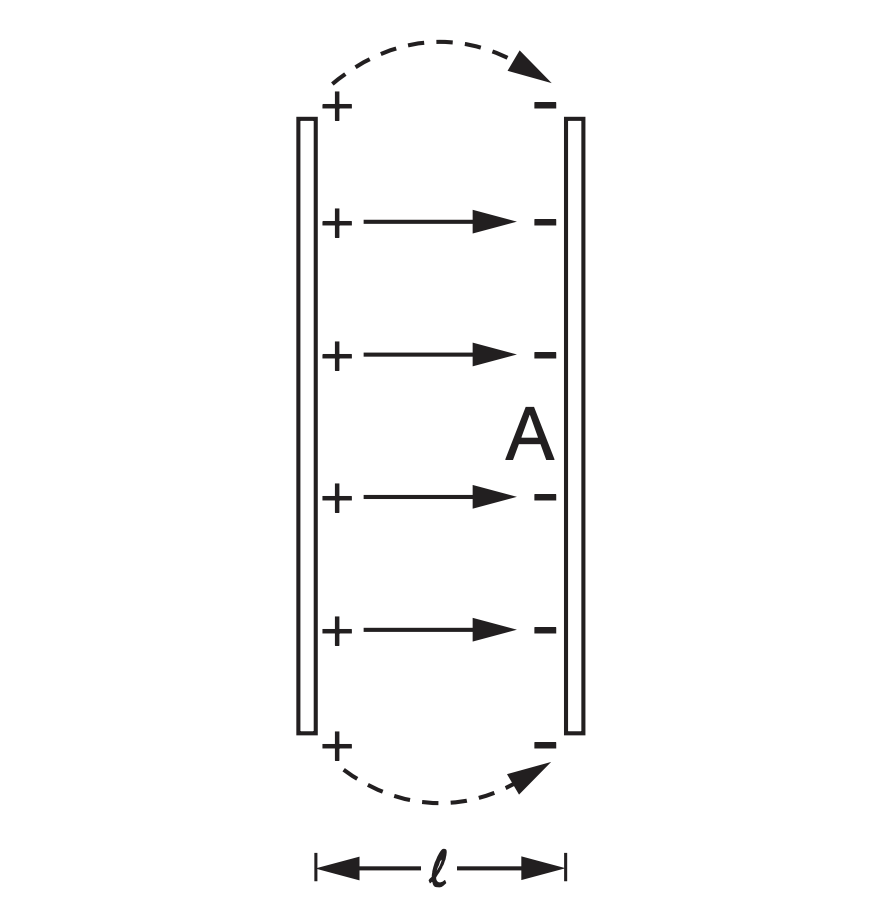
\includegraphics[scale=0.1]{Images/Plattenkondesator.png}
        \end{center}
        2) Kugelkondensator:
        \[U = \frac{Q}{4\pi\varepsilon_0}\Bigl(\frac{1}{r_1} - \frac{1}{r_2}\Bigr)\]
        \[C = \frac{Q}{U} = 4\pi\varepsilon_0\Bigl(\frac{r_1 r_2}{r_2 - r_1}\Bigr)\]
        falls $r_2 \rightarrow \infty$, dann $C = 4\pi\varepsilon_0\,r_1$.
        \begin{center}
            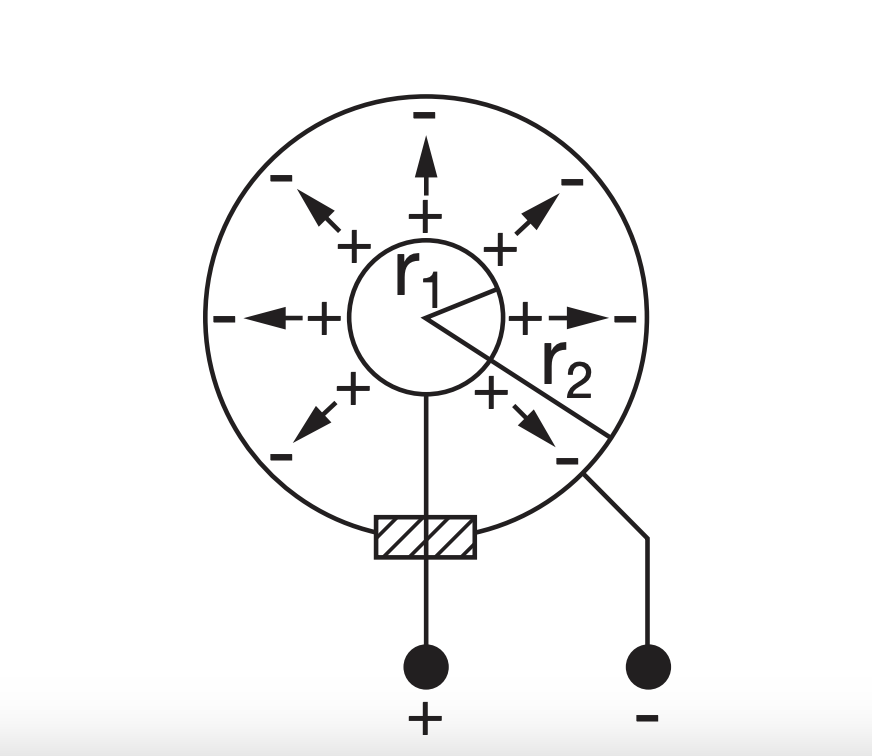
\includegraphics[scale=0.1]{Images/Kugelkondensator.png}
        \end{center}
        
         E-Feld, falls wir vom Feld einer Platte sprechen:
        \[\vec E = \frac{U}{2d}\]
    
    \subsubsection{Dielektrikum}
        Zwischen zwei Kondensatorplatten wird ein isolierendes Material eingeschoben, Spannung sinkt und Kapazität steigt.
        
        \[\vec D_m = \varepsilon\,\varepsilon_0\,\vec E_m\]
        wobei $\varepsilon$ die Dielektrizitätskonstante des Materials ist.\\
        Unterscheidung:\\
        1) ferroelectric: $\varepsilon > 1$, temperatur- und feldunabhängig\\
        2) paraelektrisch: $\varepsilon > 1$, temperaturabhängig und feldunabhängig\\
        3) ferromagnetisch: $\varepsilon \gg 1$, temperatur- und feldabhängig
        
    \subsubsection{Ladevorgang eines Kondensators}
        Es dauert eine gewisse Zeit, bis ein Kondensator geladen ist:
        \[U_0 = U_R + U_C\]
        \[U_R = I R\]
        \[I = I_0\,e^{-\frac{t}{RC}}\]
        bei $t = 0 \rightarrow Q = 0$, wächst aber asymptotisch gegen $Q_0 = C\,U_0$
        \begin{center}
            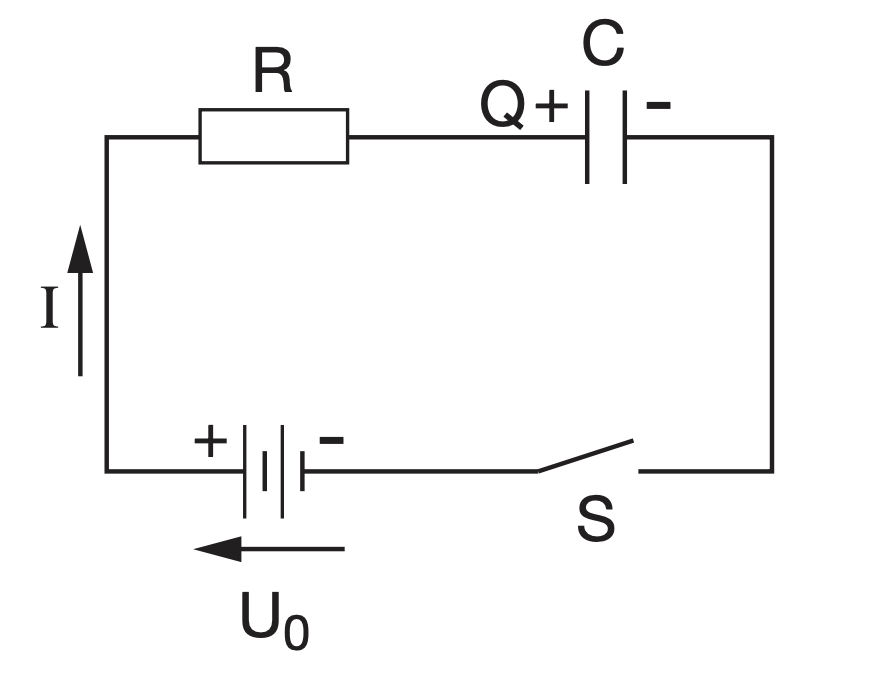
\includegraphics[scale=0.1]{Images/Ladevorgang Kondensator.png}
        \end{center}
    
    \subsubsection{Energie des elektrischen Feldes/Plattenkondensator im Dielektrikum}
        \[W = \frac{1}{2}\varepsilon_0\,\frac{A}{l}U^2 = \frac{1}{2}\varepsilon_0\,(A\,l)\frac{U^2}{l^2} = \frac{1}{2}\varepsilon_0\,E^2\,V\]
        Energiedichte:
        \[\rho_{el} = \frac{W}{V} = \frac{1}{2}\varepsilon_0\,E^2 = \frac{1}{2}(\vec D \cdot \vec E)\]
        \begin{center}
            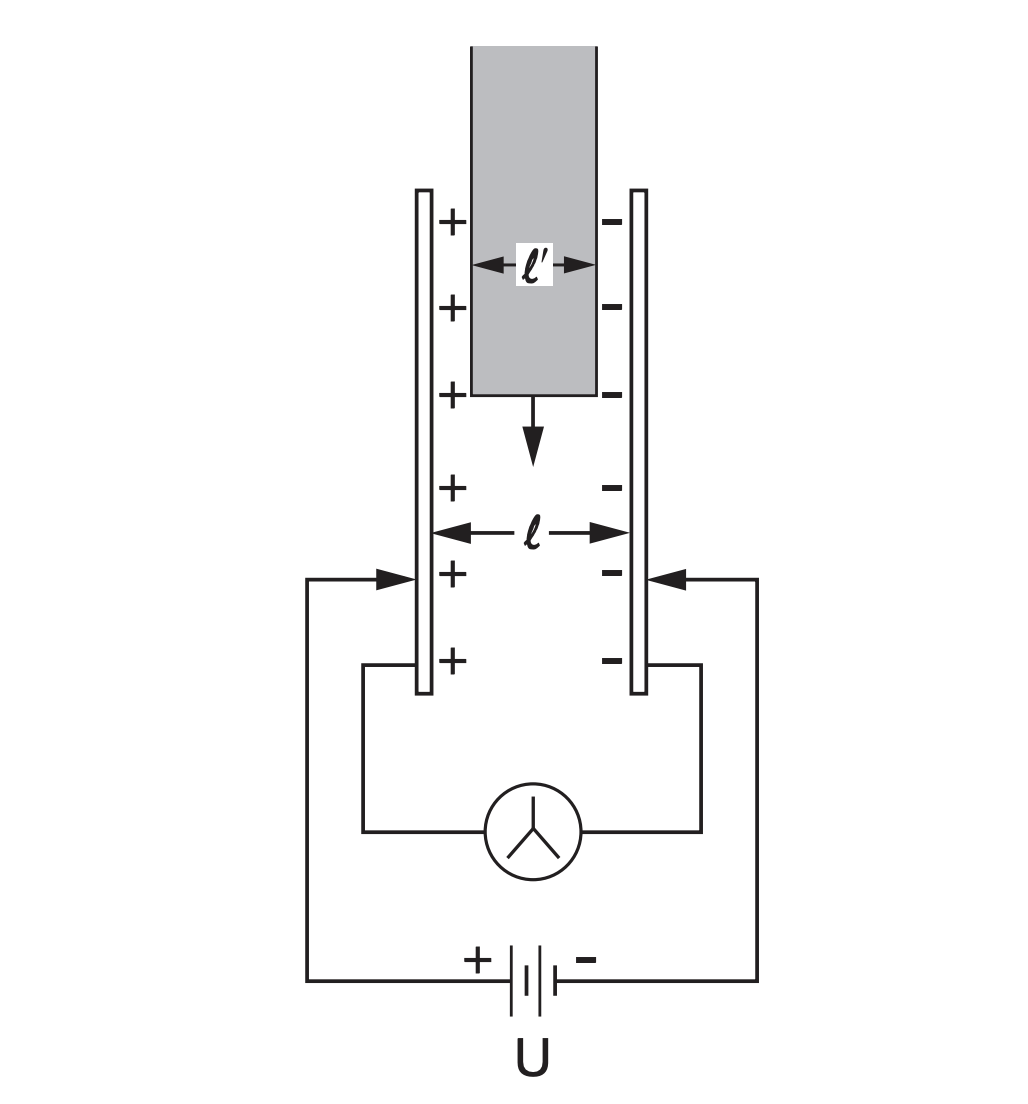
\includegraphics[scale=0.1]{Images/Dielektrikum.png}
        \end{center}
        \[W_{\text{tot}} = W_{el} + W_{pot}\]

%=====================================================================================================================
\subsection{Leiter}
\subsubsection{Ohmsche Leiter}
    Bei Ohmschen Leitern gilt:
    \[ I \sim U, I = \frac{U}{R}\]
    \begin{center}
        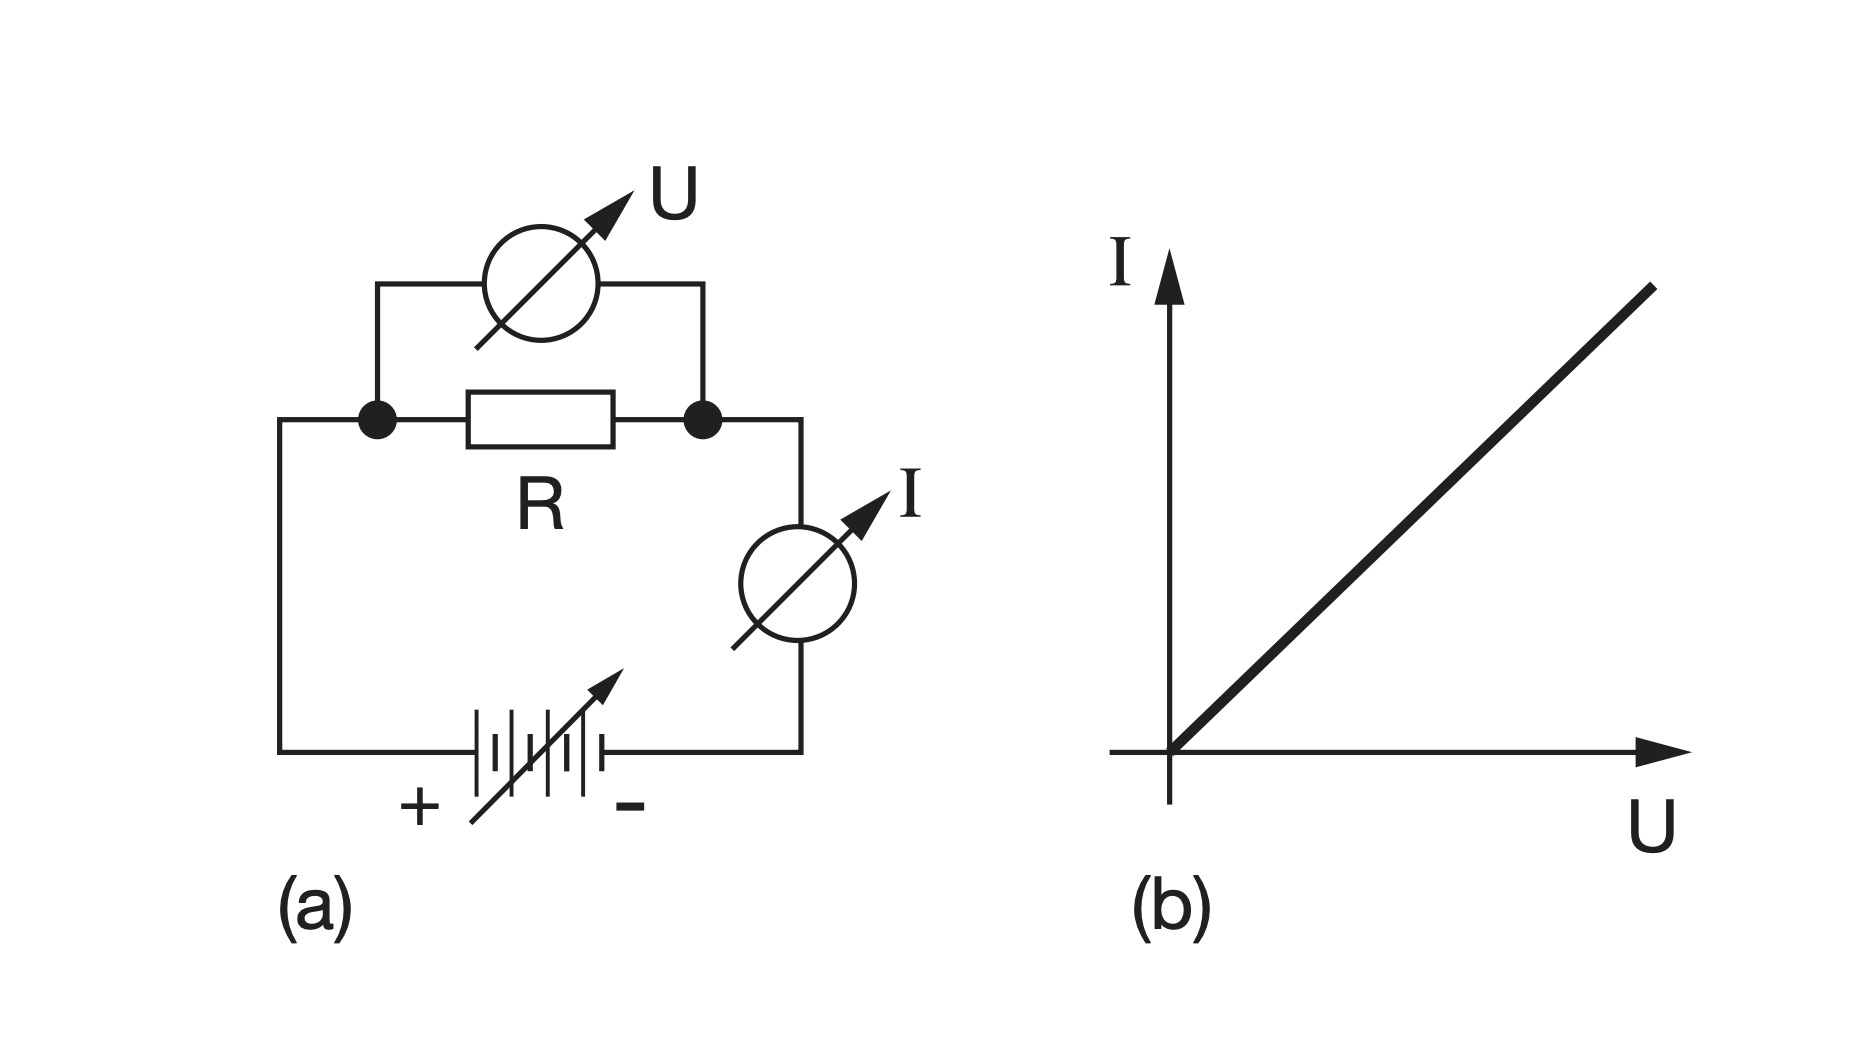
\includegraphics[scale=0.15]{Images/NichgtOhnscheLeiter.png}
    \end{center}
    \subsubsection{Klassifizierung von Leiter}
    \hl{nach Grösse:}
        \[R = \rho\frac{l}{A}\]
        wobei l = Leiterlänge, A = Leiterquerschnitt und $\rho$ der spezifische Widerstand [$\Omega\text{m}$]\\
        
        Spezifische Leitfähigkeit (Conductivity) :
        \[K = \frac{1}{\rho}\]
        $\rho < 10^{-8} \Omega\text{m = guter Leiter}$\\ 
        $ \rho \approx 10^{-8} \Omega\text{m = Halbleiter }$\\$\rho > 10^8 [\Omega\text{m] = gute Isolatoren}$\\

        Leitwert:\\
        \[\frac{1}{R}\]

    \hl{nach Temperatur}\\
        In metallischen Leitern werden die Elektronen an den schwingenden Atomen gestreut, in Bewegung gebremst und gehindert.
        
        \[\rho(T) = \rho_0[1+\alpha(T - T_0)]\]
        $\rho_0$ = spezif. Widerstand,\\
        $T_0$ = Bezugstemp.\\
        $\alpha$ = Temp.koeffizient des spez. Widerstands $[1/K]$.\\\\
        
        \hl{Supraleiter}\\
            Falss bei manchen metallischen Leitern der Widerstand bei einer charakterisitschen Temp. auf 0 fällt\\
        
        \hl{Halbleiter}\\
            Spezifischer Widerstand fällt exponentiel mit steig. Temp. Bei tiefen Temp. gute Isolatern, da alle Elektronen an der Gitterbindung beteiligt. 
            
        \begin{center}
            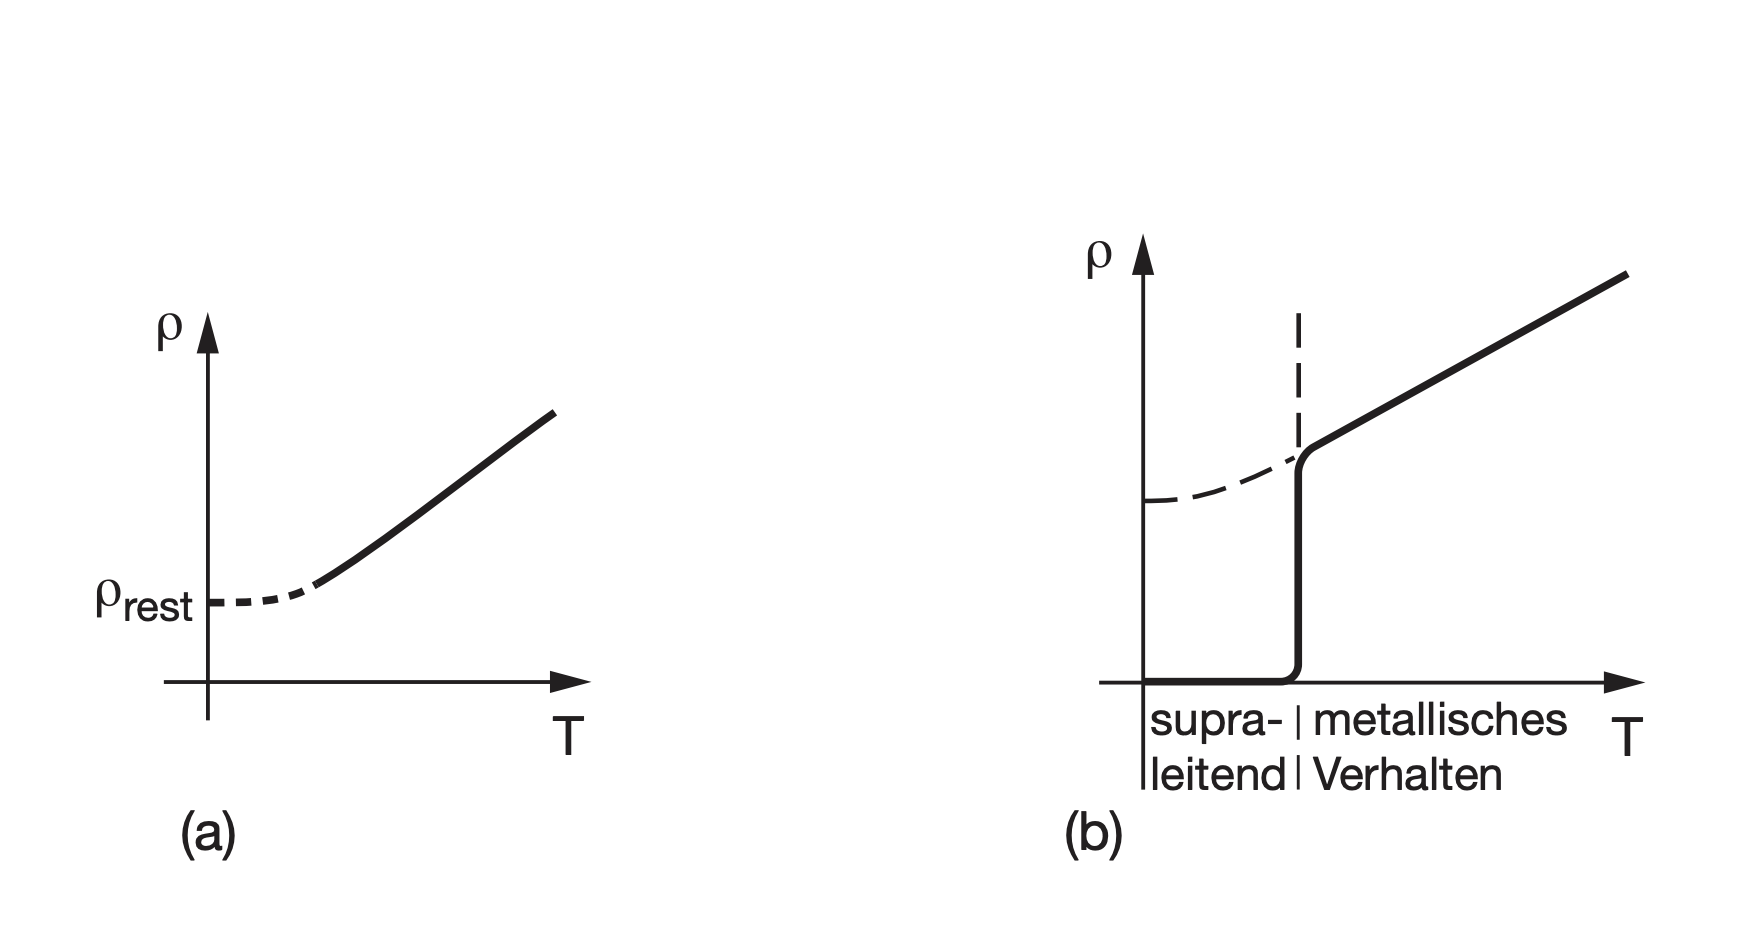
\includegraphics[scale=0.2]{Images/Klassifizierung.png}
        \end{center}
        \begin{center}
            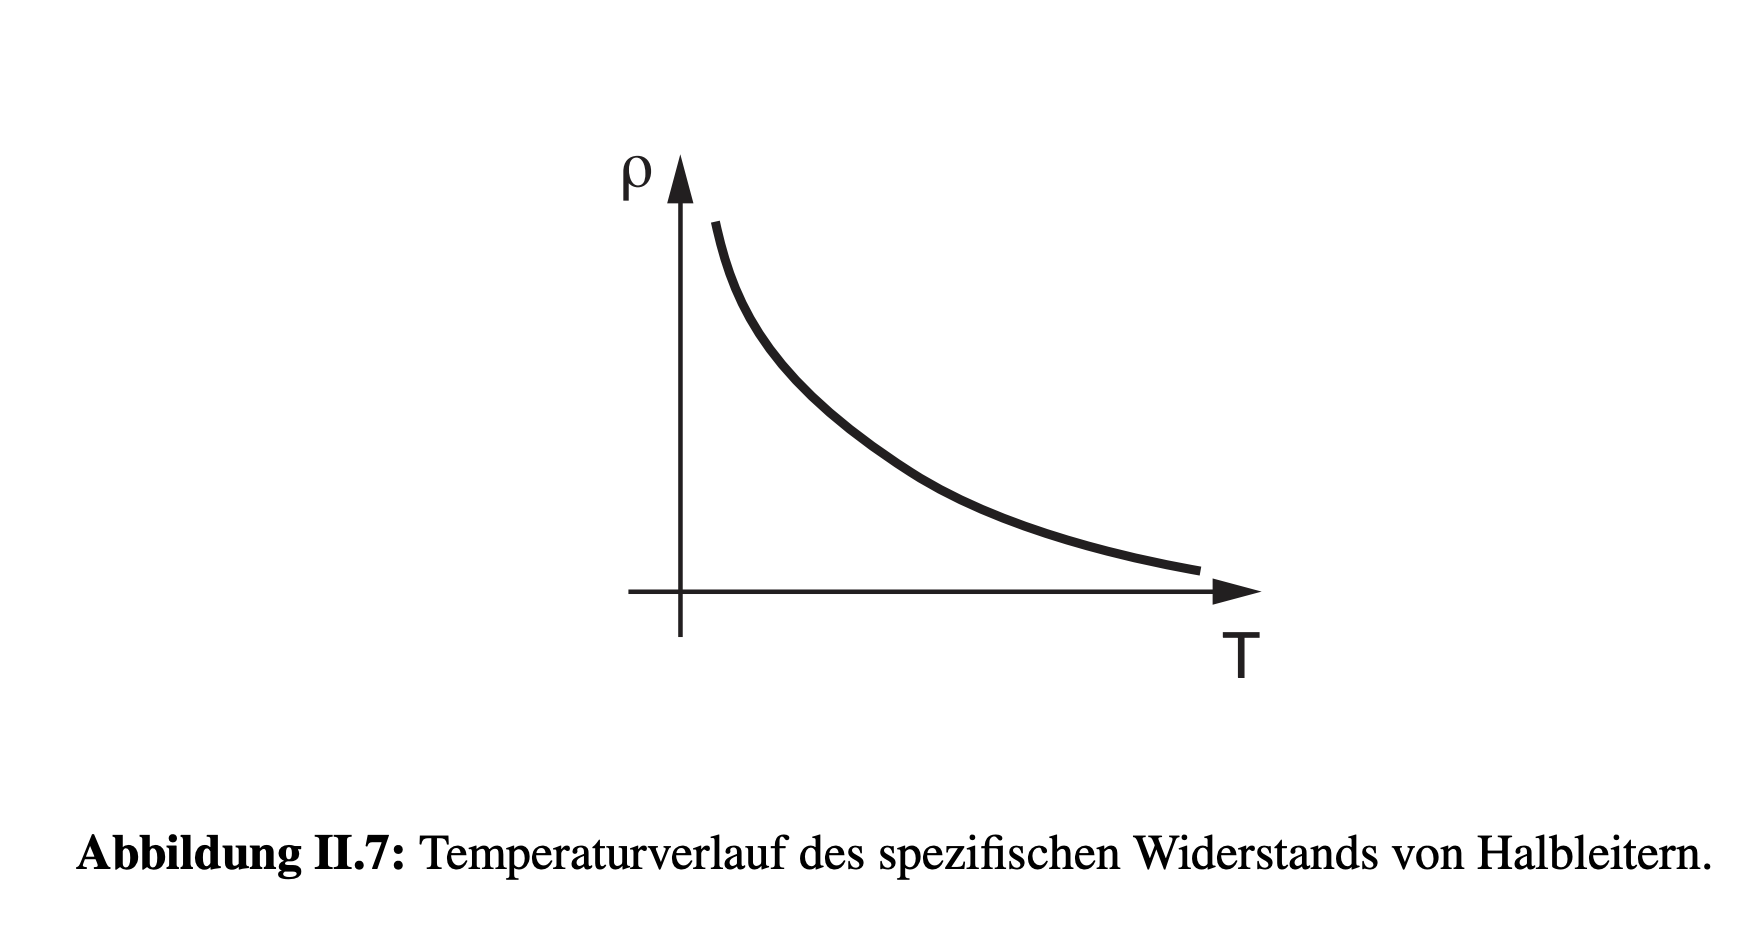
\includegraphics[scale=0.2]{Images/Tempverlauf von Halbleiter.png}
        \end{center}
    
%=====================================================================================================================
\subsubsection{Nicht-ohmsche Leiter}
Proportionalität zwischen U und I gilt \hl{nicht}
\[R_{diff} = \frac{dU}{dI}\]
\begin{center}
    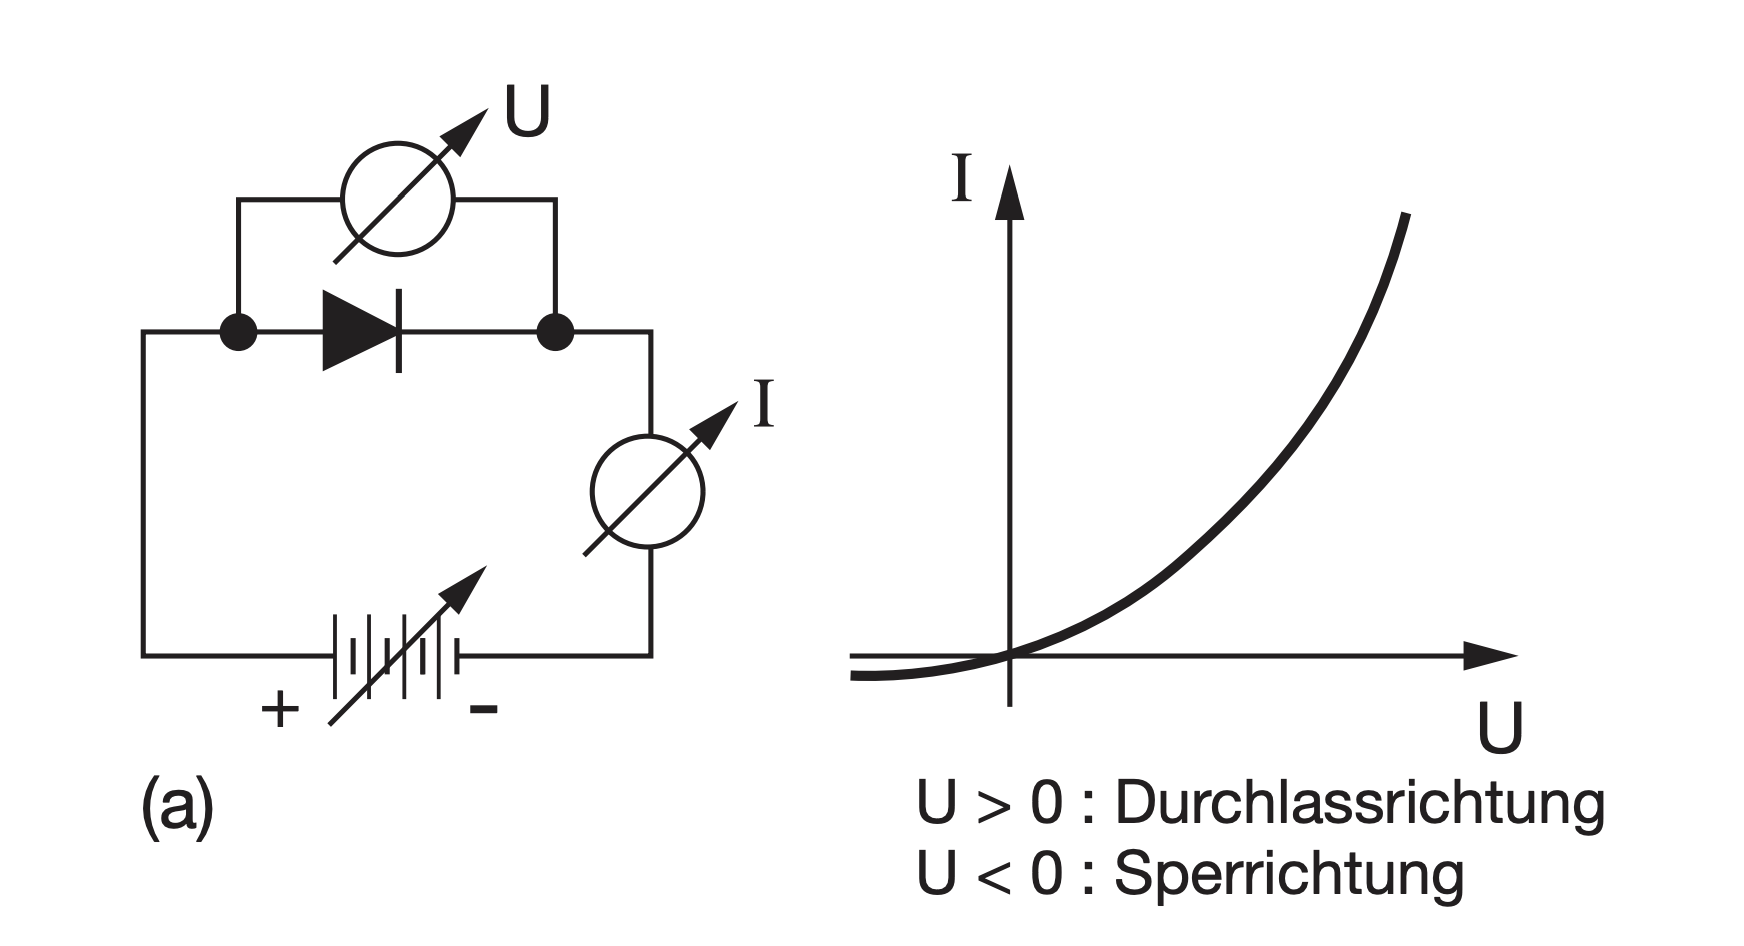
\includegraphics[scale=0.1]{Images/Ohmscheleiter.png}
\end{center}

%=====================================================================================================================
\subsection{Schaltungen}
\subsubsection{Kirchhoffsche Regeln}
\hl{Knotenregel:}
\[\sum_k I_k = 0\]
Bei einem Knotenpunkt(K) gilt $I_{zu} = I_{ab}$. \\
\hl{Maschenregel:}
\[\sum_i U_i = \sum_k I_k R_k = \sum_k \frac{Q_k}{C_k}\]
Die Summe aller Teilspannung = Spannung der Quelle: $U = U_1 + U_2 + \dots + U_n$


%=====================================================================================================================
\subsubsection{Serienschaltung/Reihenschaltung}
\[R_{tot} = \sum_i R_i\]
$U_0 = I(R_1 + R_2) = IR_{tot}, R_{tot} = R_1 + R_2$
\[U_{ges} = U_1 + U_2 + \dots + U_n\]
\[I_{ges} = I_1 = I_2 = \dots = I_n\]
\[\frac{Q}{C} = \frac{Q}{C_1}+\frac{Q}{C_2}\]
\[\frac{1}{C} = \frac{1}{C_1} + \frac{1}{C_2}\]

%=====================================================================================================================
\subsubsection{Parallelschaltung}
\[\frac{1}{R_{tot}} = \sum_i \frac{1}{R_i}\]
\[I_{ges} = I_1 + I_2 = \frac{U}{R_1} + \frac{U}{R_2} = U\frac{1}{R_{tot}}\]
\[\frac{1}{R_{tot}} = \frac{1}{R_1} + \frac{1}{R_2} = \frac{R_1 + R_2}{R_1R_2}\]
\[U_{ges} = U_1 = U_2 = \dots = U_n\]
\[CU_0 = C_1U_0 + C_2U_0\]
\[C = C_1 + C_2\]


%=====================================================================================================================
\subsection{Hall Effekt}
\[U_H = \frac{A_H \cdot I \cdot B}{d}\]
\begin{center}
    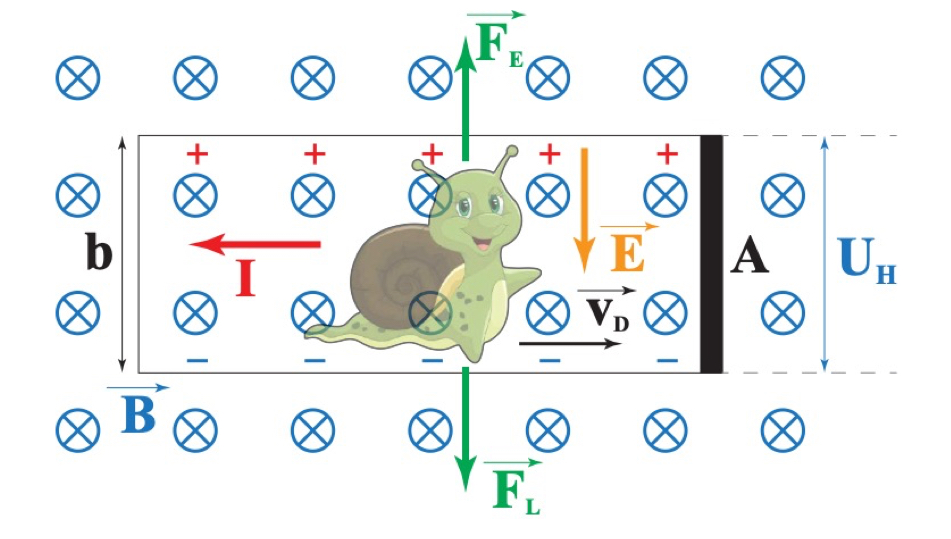
\includegraphics[scale=0.15]{Images/Halleffekt.jpg}
\end{center}

\columnbreak
%%%%%%%%%%%%%%%%%%%%%%%%%%%%%%%%%%%%%%%%%%%%%%%%%%%%%%%%%%%%%%%%%%%%%%%%%%%%%%%%%%%%%%%%%%%%%%%%%%%%%%%%%%%%%%%%%%%%%%
\section{Elektrisches Feld/ Potential/ Fluss}
Elektrische Felder entstehen dort, wo elektrische Spannung herrscht.

%=====================================================================================================================
\subsection{Elektrische Feldstärke E/D}
    Homogenes elektrisches Feld zwischen zwei ebenen geladenen Platten (mit Abstand $l$ und Plattenfläche $A$):
    
    \[\vec E = \frac{U}{l}\hat{e} = v \cdot \vec B \]
    wobei $\hat{e}$ = Einheitsvektor und [E] = V/m
    \[E_{achse} = |\vec E|\cos\alpha \]
    wobei $\alpha$ der Winkel zwischen $\vec E$ und der jeweiligen Achse ist.\\
    Superpositionsprinzip von zwei E-Feldern verschiedener Herkunft:
    \[\vec E = \vec E_1 + \vec E_2\]\\
    E-Flussdichte:
    \[\eqbox{\vec D = \frac{Q}{A} \hat{e}}\] 
        D = [$\frac{C}{m^2}$]\\
        Im Vakuum gilt: 
        \[ \vec D = \varepsilon_0 \vec E\]
        E und D sind Vektoren, die tangential zu jedem Punkt der Feldlinien stehen.
    \begin{center}
        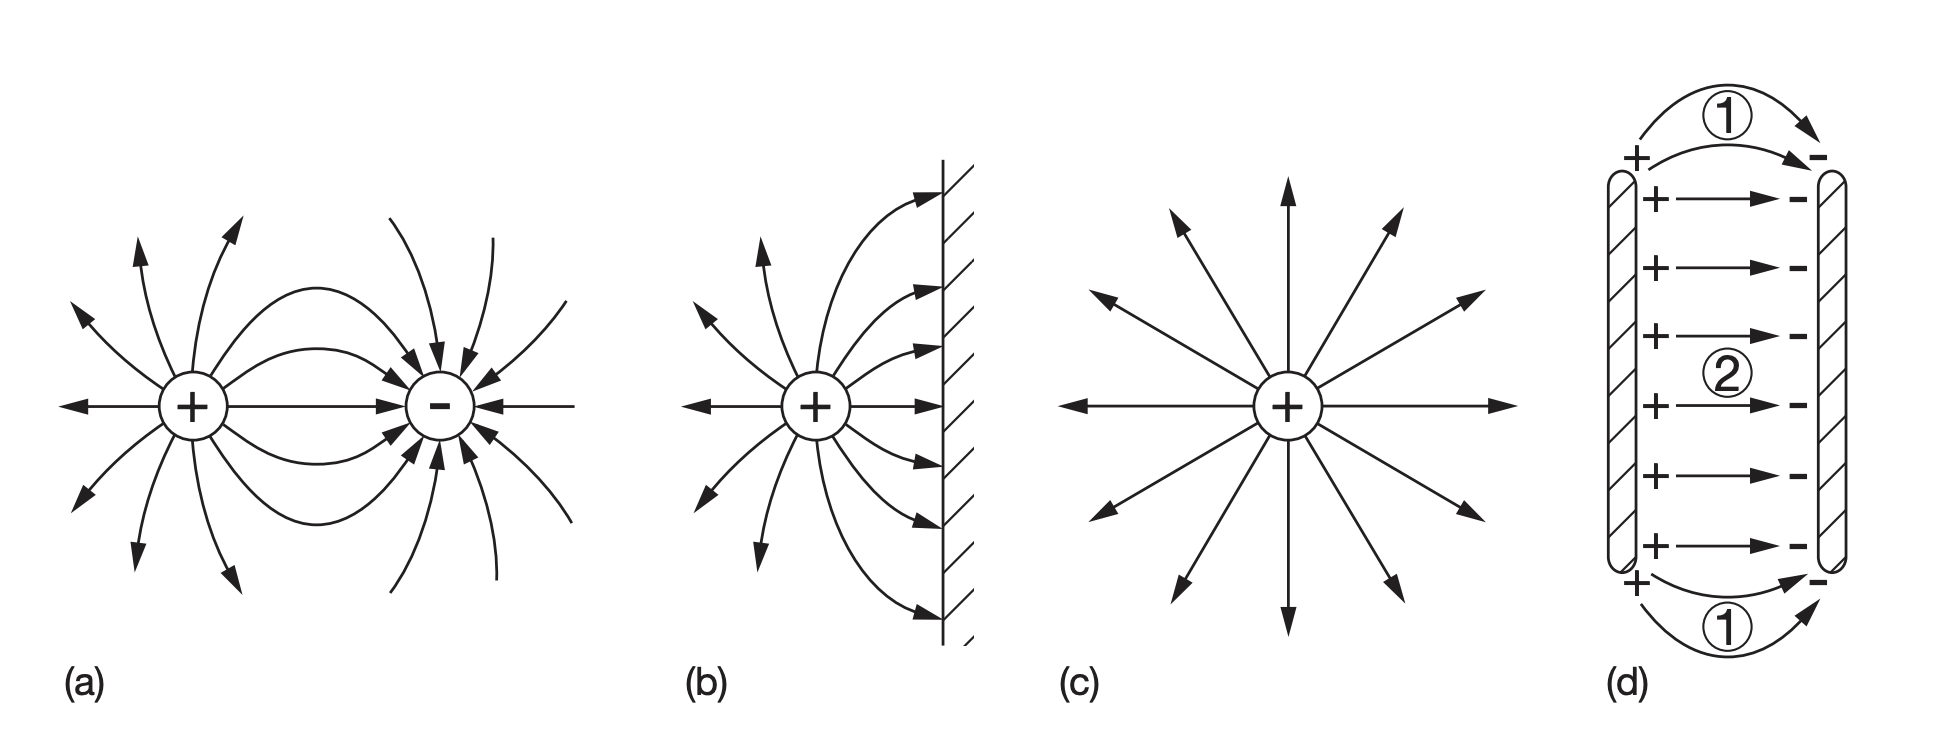
\includegraphics[scale=0.1]{Images/ElektrischeFeld.png}
    \end{center}


%=====================================================================================================================
\subsection{Elektrisches Potential}
    Spannungsdifferenz zwischen beiden Platten/Punkten/Leiter = Potentialdifferenz:
    \[U_{P_0 P} = - \int_{P_0}^P \vec E \cdot d\vec s = - \int_{P_0}^P E \cos\alpha \, ds = \phi(P) - \phi(P_0)\]
    Minus, da gegen die Feldlinien gelaufen\\
    
    \hl{Geschlossener Weg (mit konst. M-Feld):}\\
    \[\oint\vec{E}d\vec{s}=0\]\\
    Zusammenhang zwischen Feld und Potential:
    \[\vec E = - \frac{d\phi(P)}{ds} = - \nabla\phi\]

%=====================================================================================================================
\subsection{Coulomb-Potential}
    \[\phi(r) = \frac{1}{4\pi\varepsilon_0}\frac{Q}{r}\]
    E-Feld einer Punktladung (auf Kugel):
    \[\vec E = \frac{1}{4\pi\varepsilon_0} \frac{Q}{r^2} \,\hat{e}_r\]
    Bei einer Ansammlung von Punktladungen:
    \[\phi(r) = \frac{1}{4\pi\varepsilon_0}\sum_i \frac{Q_i}{r_i}\]
    \begin{center}
        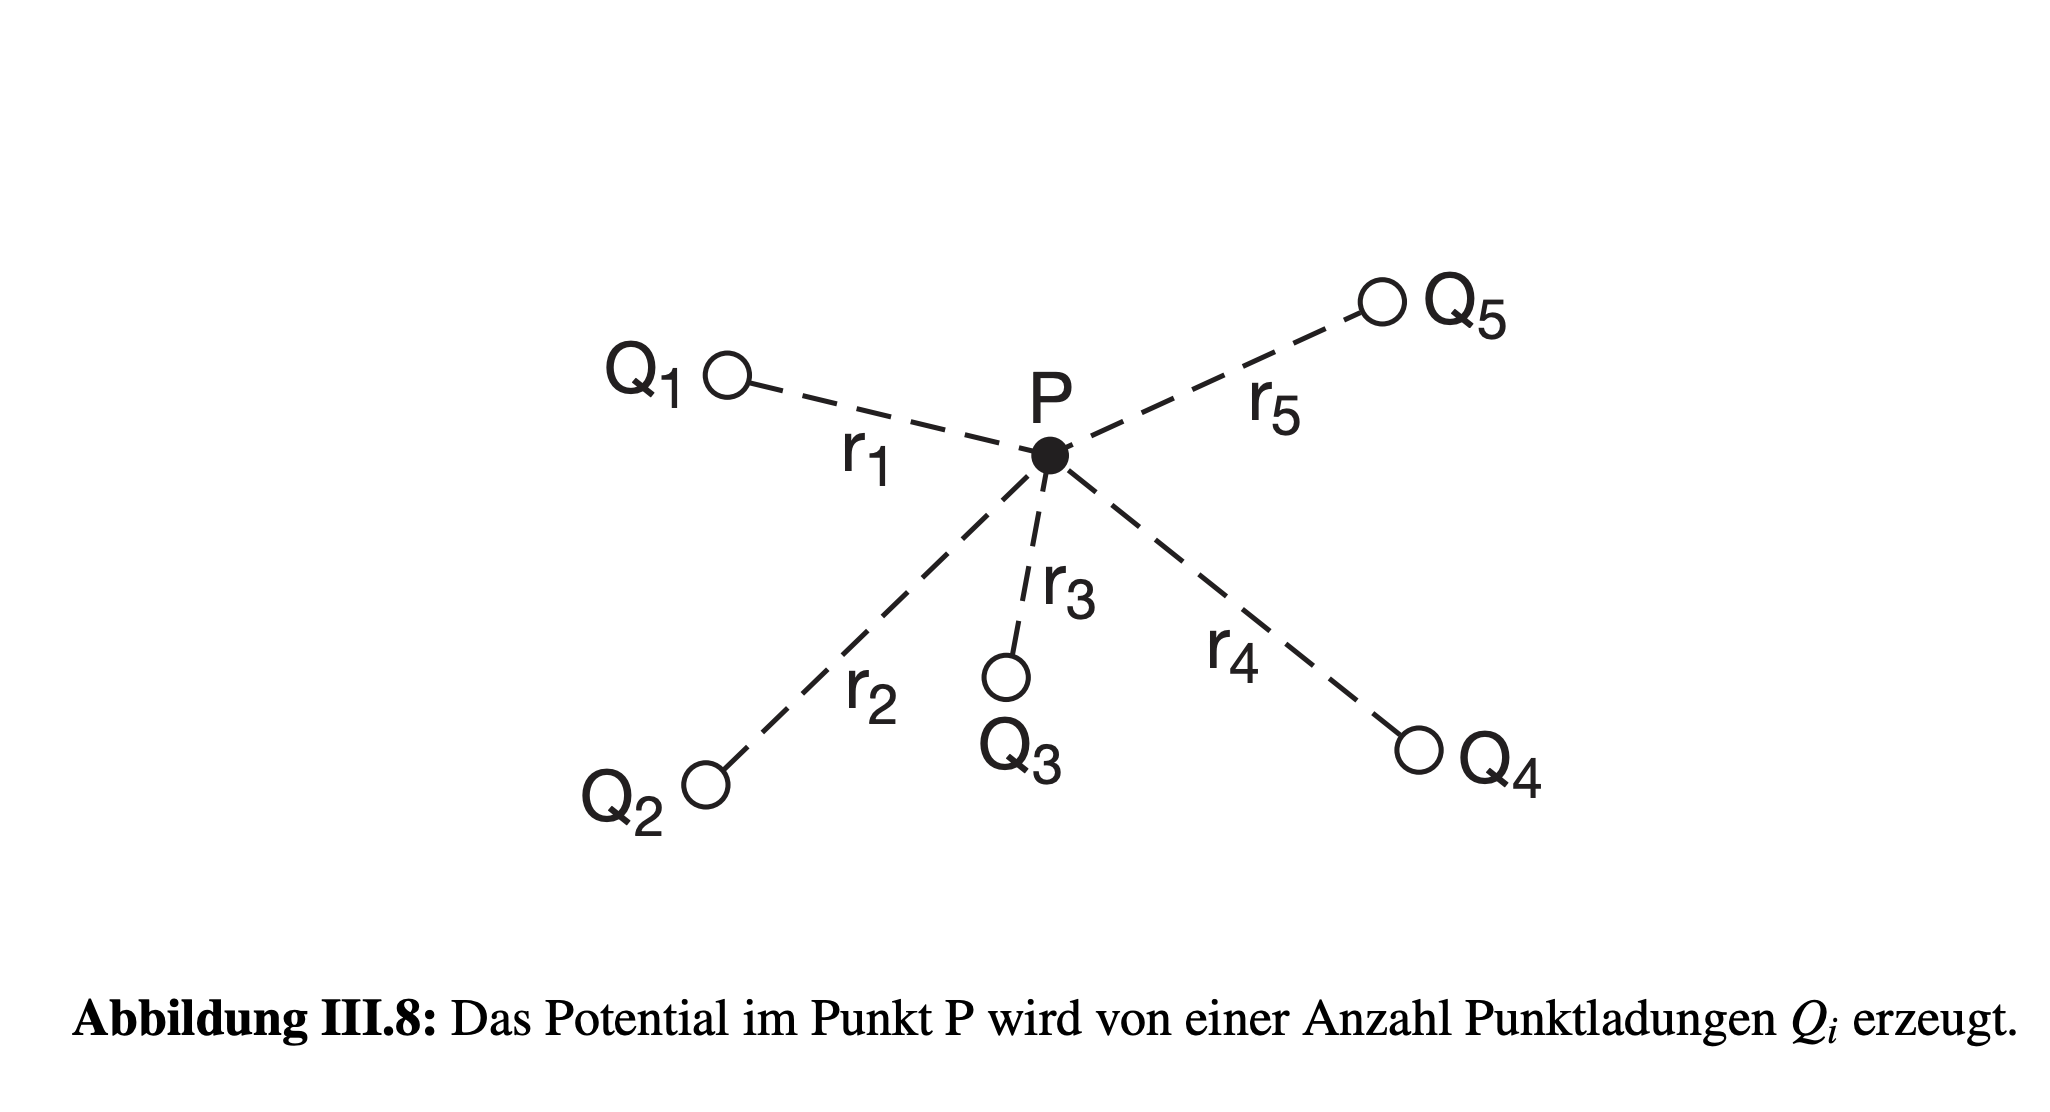
\includegraphics[scale=0.2]{Images/Punktladungen.png}
    \end{center}
    Potential einer räumlichen Ladungsverteilung:
    \[\phi(r) = \frac{1}{4\pi\varepsilon_0} \int \frac{\rho(\mathbf{r}')\,dV'}{|\mathbf{r} - \mathbf{r}'|}\]
    \begin{center}
        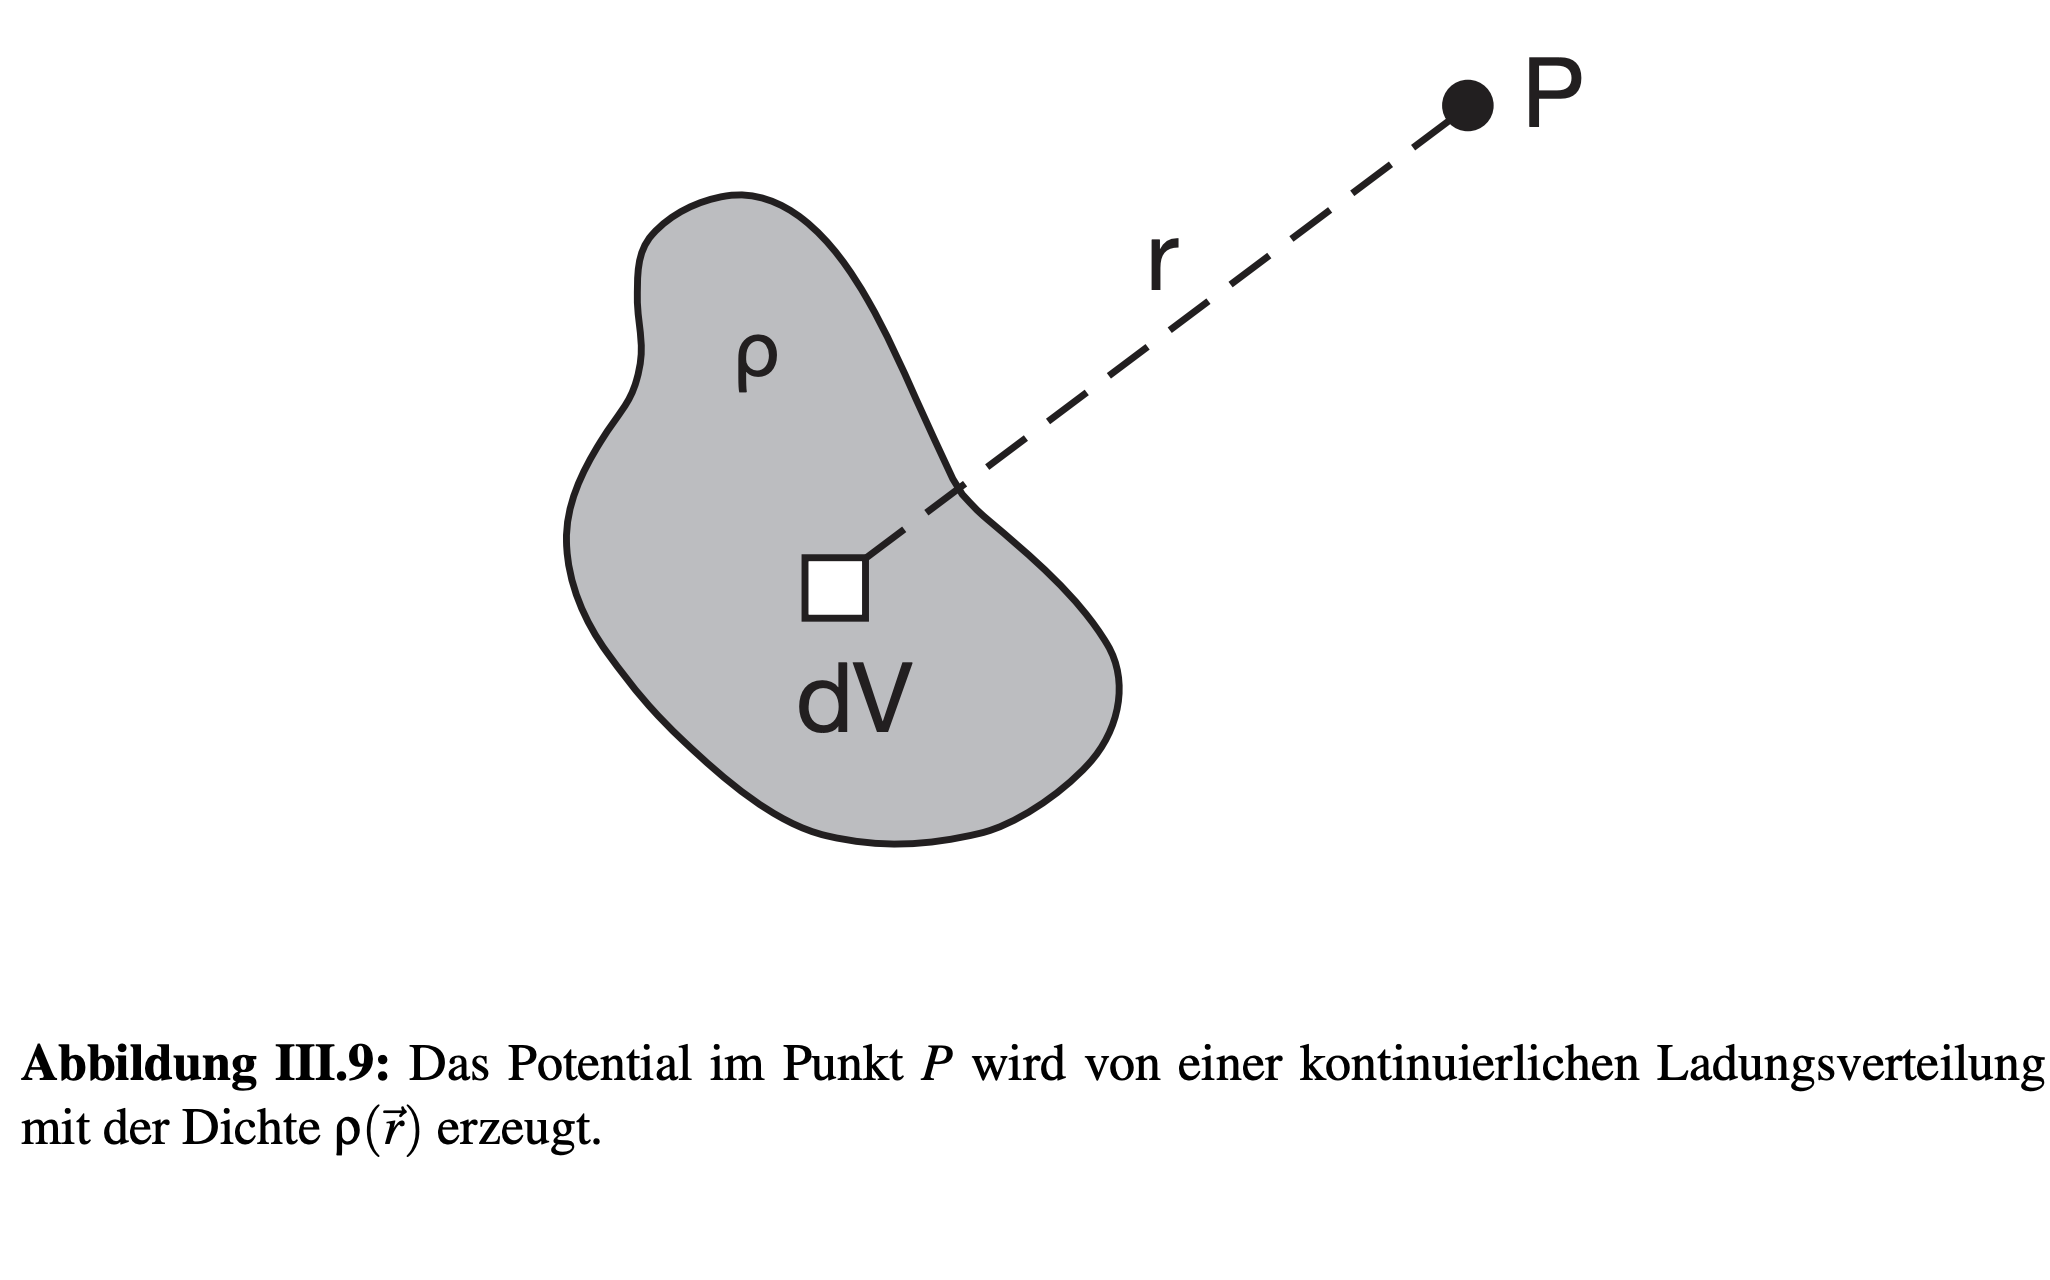
\includegraphics[scale=0.2]{Images/Ladungsverteilung.png}
    \end{center}

%=====================================================================================================================
\subsection{Potential und Feld eines elektrischen Dipols}
    Elektrisches Dipolmoment: \\
    \[\vec p = Q \,\vec l\]\\
    Beispiel: zwei Punktladungen mit entgegengesetzen Ladungen $\pm Q$:
    \[\phi_{\text{dip}} = \frac{1}{4\pi\varepsilon_0} \left(\frac{Q}{r_1} - \frac{Q}{r_2}\right) = \frac{Q}{4\pi\varepsilon_0}\,\frac{r_2 - r_1}{r_1 r_2}\]
    \[= \frac{1}{4\pi\varepsilon_0}\,\frac{Q\,l\cos\alpha}{r^2}\]
    \begin{center}
        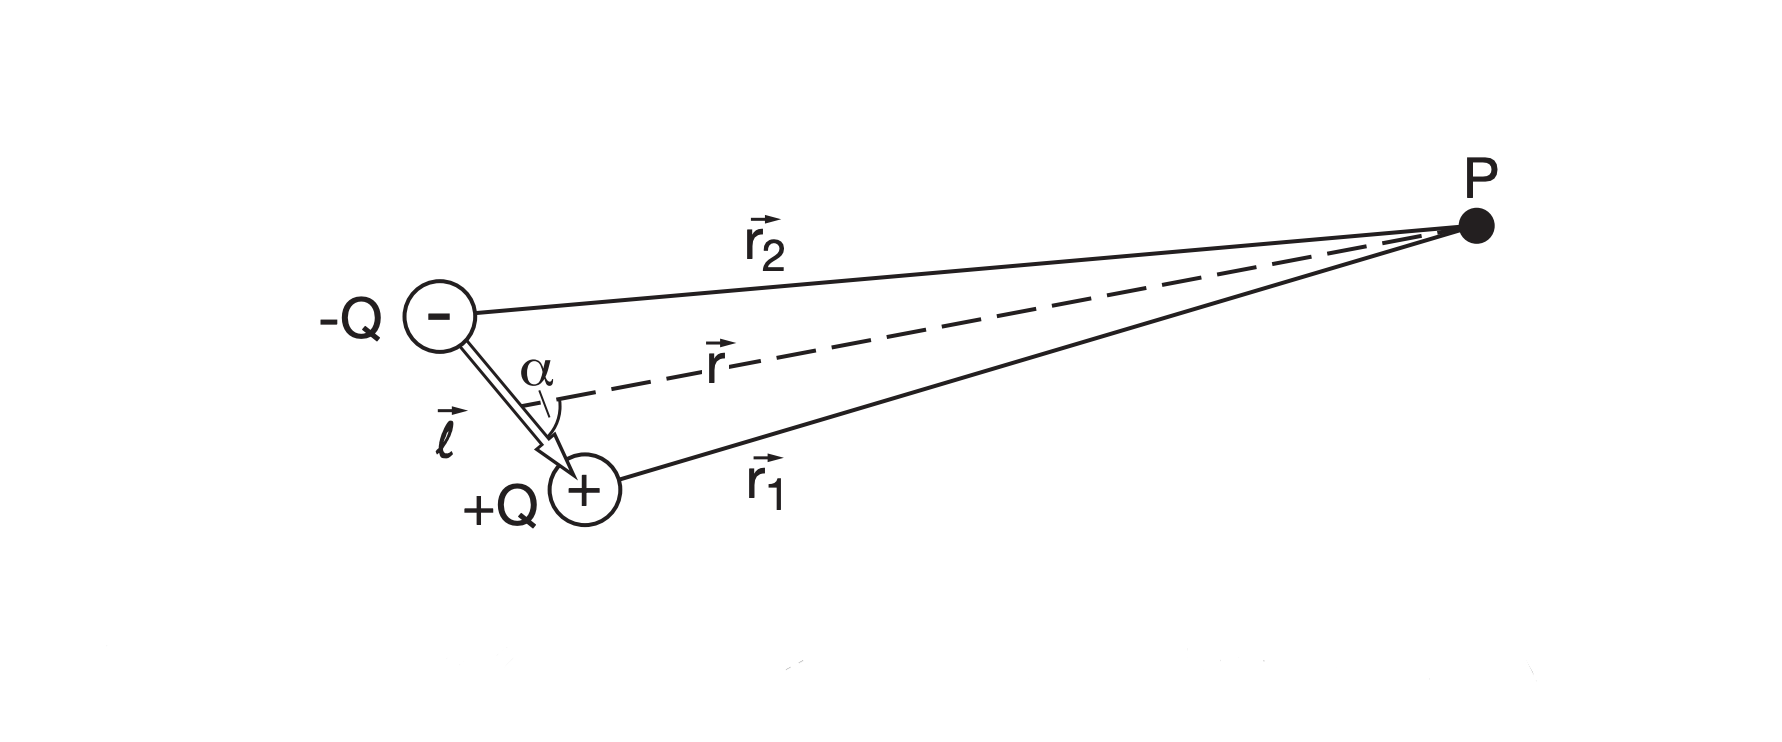
\includegraphics[scale=0.15]{Images/PotimPuntP.png}
    \end{center}

    
%=====================================================================================================================
\subsection{Elektrischer Fluss}
    Feldlinien werden durch Richtung und Feldstärke charakterisiert. Feldlinien gehen vom \hl{positiv} zum \hl{negativ}\\
    
    \[\Psi = \int d\Psi = \int \vec E \cdot d\vec A \]
%=====================================================================================================================
\subsection{Guass'sche Satz}
    Bei Ladungsverteilung innerhalb einer geschlossenen Fläche gilt:\\
    \[\eqbox{\frac{1}{\epsilon_0}\oint\rho dV = \oint \vec E \cdot d\vec A = \frac{1}{\varepsilon_0} \int \rho \, dV}\]
    Fluss durch geschlossene Fläche = von der Fläche umschlossene elektrische Ladung / $\varepsilon_0$.
    Daraus folgt die dritte Maxwell-Gleichung:
    \[\nabla \cdot \vec E = \frac{1}{\varepsilon_0}\rho,\quad \nabla \cdot \vec D = \rho\]
    
    \subsubsection{Anwendung}
    1) Feld einer linearen Ladungsverteilung (mit linearer Ladungsdichte $\lambda$):
    \[\oint \vec E \cdot d\vec A = \frac{1}{\varepsilon_0}\,\lambda\,l,\quad E = \frac{1}{2\pi\varepsilon_0}\,\frac{\lambda}{r} = \frac{1}{2\pi \varepsilon_0} \frac{Q}{l\,r}\]
    \begin{center}
        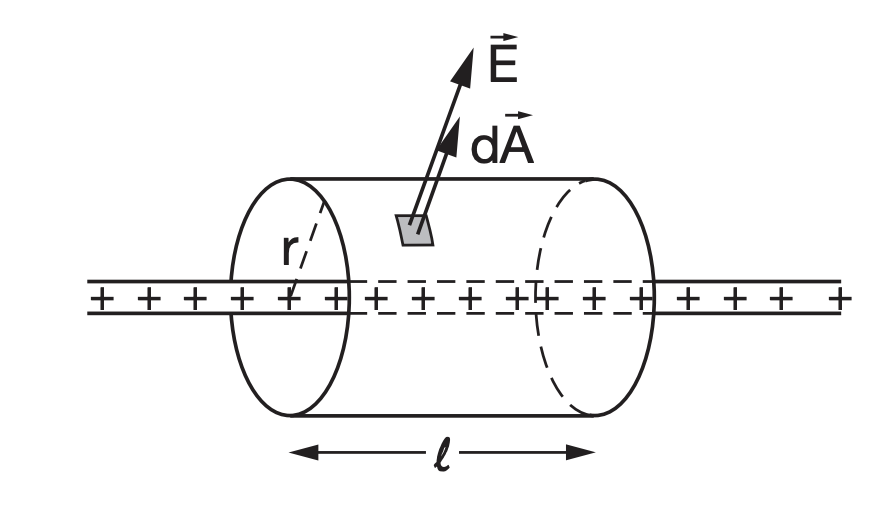
\includegraphics[scale=0.1]{Images/linLadungs.png}
    \end{center}
    2) Elektrisches Feld einer Punktladung:
    \[\oint \vec E \cdot d\vec A = \frac{Q}{\varepsilon_0},\quad E = \frac{1}{4\pi\varepsilon_0}\,\frac{Q}{r^2}\]
    3) Fläche Ladungsverteilung
    \[\vec E = \frac{\sigma}{2\varepsilon_0} \cdot \vec e\]
    (*2 weil auf beide Seite)
    


\columnbreak
%%%%%%%%%%%%%%%%%%%%%%%%%%%%%%%%%%%%%%%%%%%%%%%%%%%%%%%%%%%%%%%%%%%%%%%%%%%%%%%%%%%%%%%%%%%%%%%%%%%%%%%%%%%%%%%%%%%%%%
\section{Magnetisches Feld und Induktion}
Es gibt keine magnetischen Monopole, die kleinste magnetische Einheit ist das Dipol. (+) = Nordpol; (–) = Südpol. Feldlinien verbinden Nord- mit Südpol.\\
Magnetische Feldstärke (H):\\
\begin{tabular}[t]{@{}l l}
    im Innern einer Spule: &$H = = I\,\frac{n}{a} = I\,\frac{n}{l}$\\
    leiter schleife: &$H = \frac{1}{2} \frac{I}{r}$\\
    gerade leiter: &$H=\frac{I}{2 \pi r}$\\
    im Innnern eines dicken Kabels: &$H(r) = \frac{I}{2\pi}\,\frac{r}{R^2}$
    \end{tabular}
    \vspace{3em}

    H = $[\frac{A}{m}]$\\
    (Formeln sind Anwendungen des Durchflutungsgesetzes)
    
    
    \begin{center}
        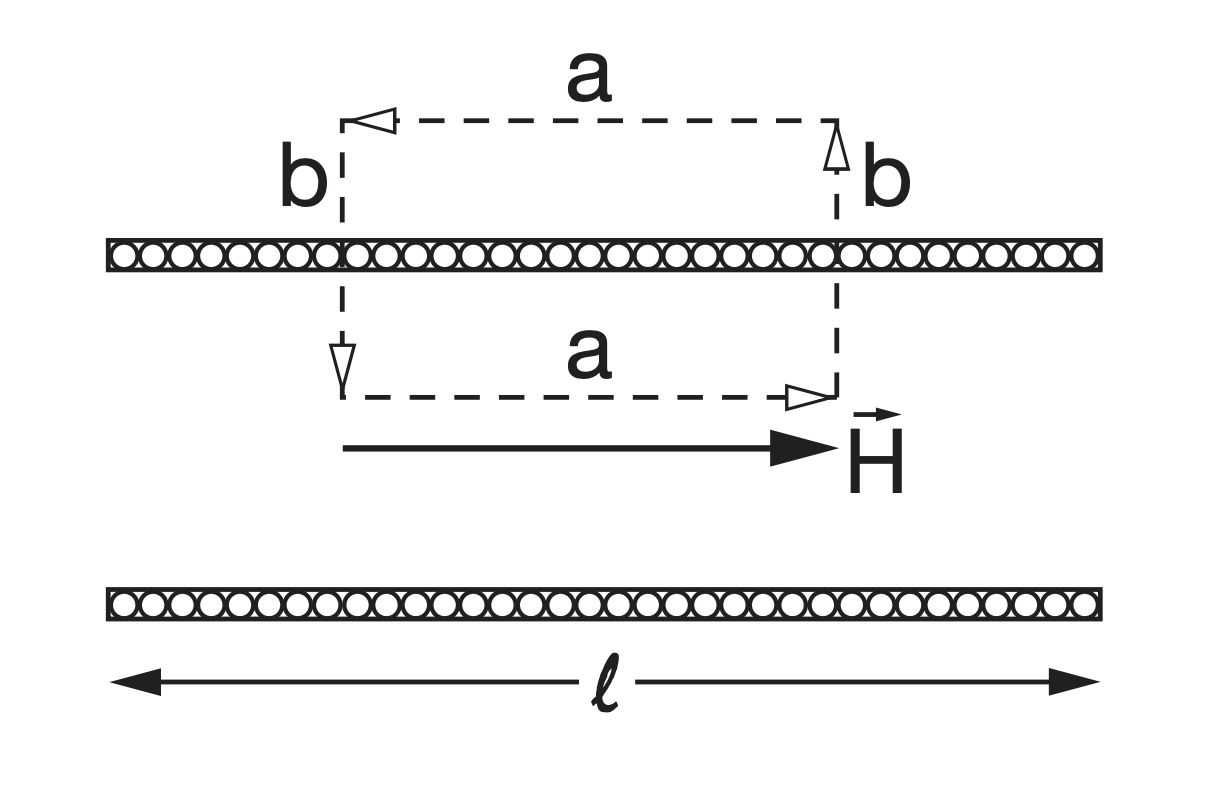
\includegraphics[scale=0.1]{Images/Spulemagfeld.png}
    \end{center}
    \begin{center}
        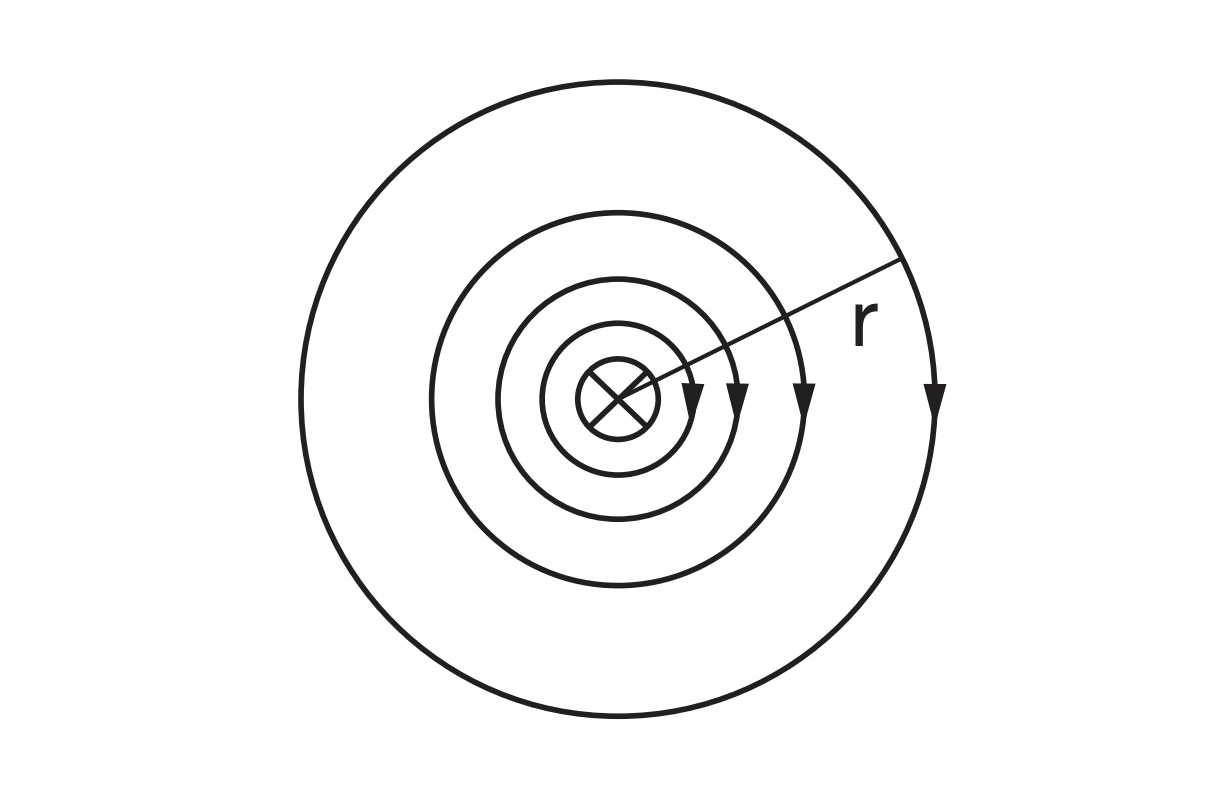
\includegraphics[scale=0.1]{Images/geraderLeiter.png}
    \end{center}
    \begin{center}
        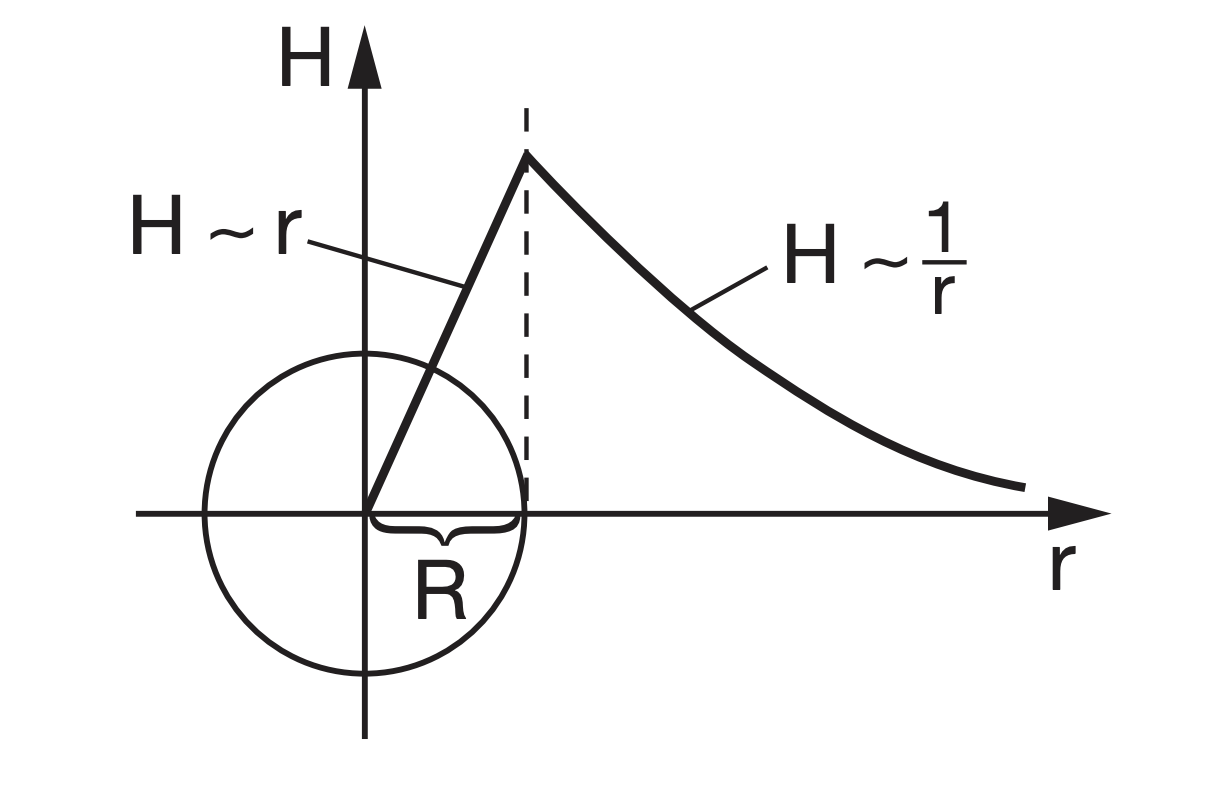
\includegraphics[scale=0.1]{Images/dickesKabel.png}
    \end{center}
    
    
%=====================================================================================================================
\subsection{Magnetischer Fluss}
    Magnetischer Fluss ($\Phi$): \\
    
    \[\Phi = \mu_0\,A\,H = A\,B\,\cos(\alpha) = \int \vec B \cdot d\vec A\]\\

    $\Phi = [Vs] = [Wb]$ (Weber)\\    
    
    Mag. Flussdichte:\\
    \[B = \frac{\Phi}{A} = \mu_0\,H\]
    \[\vec B = \mu\,\mu_0\,\vec H\]
    $B = [\frac{Vs}{m^2}]=[T]$ (Tesla)\\
    
    für homogene Felder:
    \[\Phi = B\,A\,\cos\alpha\]
    
    für inhomogene Felder:
    \[\Phi = \int \vec B \cdot d\vec A\]
    \\

    Magnetischer Fluss mit $n$ Windungen:
    \[\eqbox{n\,\Phi_{\text{eineWindung}} = \Phi_{\text{tot}} = L\,I}\]
    \\
    Kreissektor im Magnetfeld:
    \[A = \frac{a^2\,\omega\,t}{2}\]
%=====================================================================================================================
\subsection{Selbstinduktion}
    \hl{Nur bei Flussänderung!}\\
    Jede Feldspule ist eine Induktionsspule.\\
    Induktionsgesetz (Spannung → Strom):
    \[U_{ind} = -L\,\frac{dI}{dt}\]
%=====================================================================================================================
\subsection{Inkudtionsgesetz}
    \[U_{ind} = -n\,\frac{d \Phi}{dt}\]
    \[U_{ind} = - \oint \vec E \cdot d\vec s = \frac{d}{dt} \int \vec B \cdot d\vec A\]
    \[\nabla \times \vec E = \mathrm{rot}\,\vec E = - \frac{d\vec B}{dt}\]\\
    
    \hl{Lenzsche Regel:}
    Durch Änderung des magnetischen Flusses wird eine Spannung induziert, sodass der dadurch fließende Strom ein Magnetfeld erzeugt, welches der Flussänderung entgegenwirkt.

%=====================================================================================================================
\subsection{Erweiterung des Induktionsgesetzes}
    Für homogene B-Felder (Motionsinduktion):\\
    \[
    U_{\text{ind}} = (\vec{v} \times \vec{B}) \cdot \vec{l}
    \]\\
    
    Für allgemeine Fälle (bewegter Leiter + zeitveränderliches Feld):\\
    \[
    U_{\text{ind}} = \oint (\vec{v} \times \vec{B}) \cdot d\vec{l} - \frac{d}{dt} \int \vec{B} \cdot d\vec{A}
    \]

%=====================================================================================================================
\subsection{Induktivität L}
    \[L = \frac{n\,\Phi_{\text{eineWindung}}}{I} = \frac{\Phi_{\text{tot}}}{I}\]
    Für dünne, lange Spule:
    \[L = \mu_0\,n^2\,\frac{A}{l}\]\\
    $L = [\frac{Vs}{A}]=[H]$ (Henry)

%=====================================================================================================================
\subsection{Gegeninduktion}
    \hl{Nur bei Flussänderung!}\\
    Gegeninduktivität zweier langer, aufeinander gewickelter Spulen mit gleichem Querschnitt:
    \[L_{12} = \mu_0\,n_1\,n_2\,\frac{A}{l}\,\cos(\alpha) = n_2\,\frac{\Phi_{1,2}}{I}\]\\
     \( \Phi_{1,2} \) ist der von Spule 1 erzeugte Fluss durch eine Windung von Spule 2. \\

    Allgemein gilt: $L_{12} = L_{21}$. \\
    Entkopplung → $L_{12} = 0$:
    \[U_{\text{ind}} = L_{12} \,\frac{dI}{dt}\]

%=====================================================================================================================
\subsection{Spannungstoss (M-Feld $\rightarrow Strom$}
\[S = \int U_i dt = \mu_0 \frac{n A}{l} \int_a^b \vec H d \vec s\]

%=====================================================================================================================
\subsection{Biot-Savart’sches Gesetz}
    Stromverteilung in Leitungsstücken $I\,d\vec l$:
    \[\vec B = \frac{\mu_0}{4\pi} \int \frac{I\,d\vec l \times \hat{r}}{r^2}\]

%=====================================================================================================================
\subsection{Durchflutungsgesetz (Strom $\rightarrow$ M-Feld)}
    \[I_{tot} = \oint \vec H \cdot d\vec s = \int \vec j \cdot d\vec A \]
    \[\oint \vec B \cdot d\vec s = \mu_0 \,I_{\text{tot}}\]
    Dabei ist \( I_{\text{tot}} \) der gesamte eingeschlossene Strom. \\
    Für eine lange zylindrische Spule mit \( n \) Windungen pro Längeneinheit und Strom \( I \) gilt: \\
    \[H = nI\]\\
    
    (Das Ringintegral der magnetischen Feldstärke ist gleich dem elektrischen Strom, der durch die eingeschlossene Fläche fließt.)\\
    
    Da ideale Leiter und ideale Isolatoren nicht existieren, gilt:
    \[\eqbox{\oint \vec H \cdot d\vec s = \int \vec j \cdot d\vec A + \int \frac{d\vec D}{dt} \cdot d\vec A}\]\\

    (Enthält Verschiebungsstrom: berücksichtigt Änderungen des M-Feldes aufgrund von Änderungen des E-Feldes. z.B Kondensator)
    
    \begin{center}
        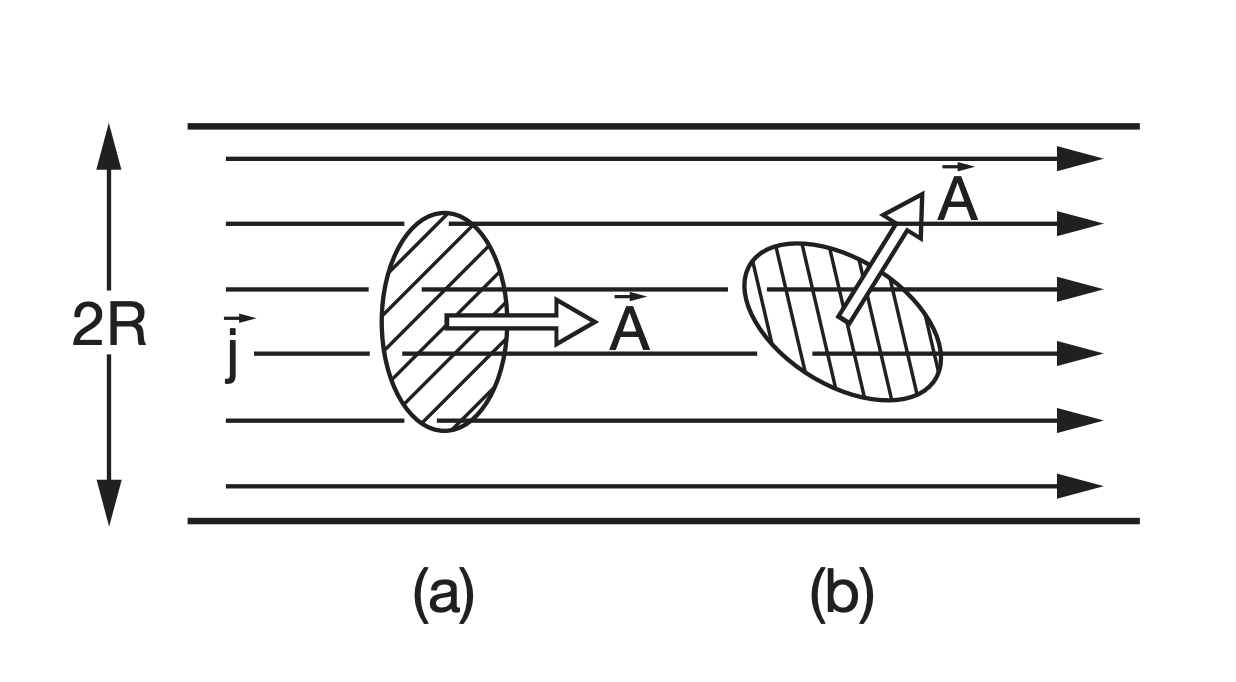
\includegraphics[scale=0.2]{Images/Durchflutungsgesetz.png}
    \end{center}
    Erste Maxwell-Gleichung (im Vakuum gilt):
    \[\mathrm{rot}\,\vec H = \frac{d\vec D}{dt}\]

\subsection{Durchflutungsgesetz}
\[
I_{\text{tot}} = \oint \vec{H} \cdot d\vec{s} = \int \vec{j} \cdot d\vec{A}
\]
\[
\oint \vec{B} \cdot d\vec{s} = \mu_0 I_{\text{tot}}
\]



%=====================================================================================================================
\subsection{Schaltkreis mit Spule}
    \begin{center}
        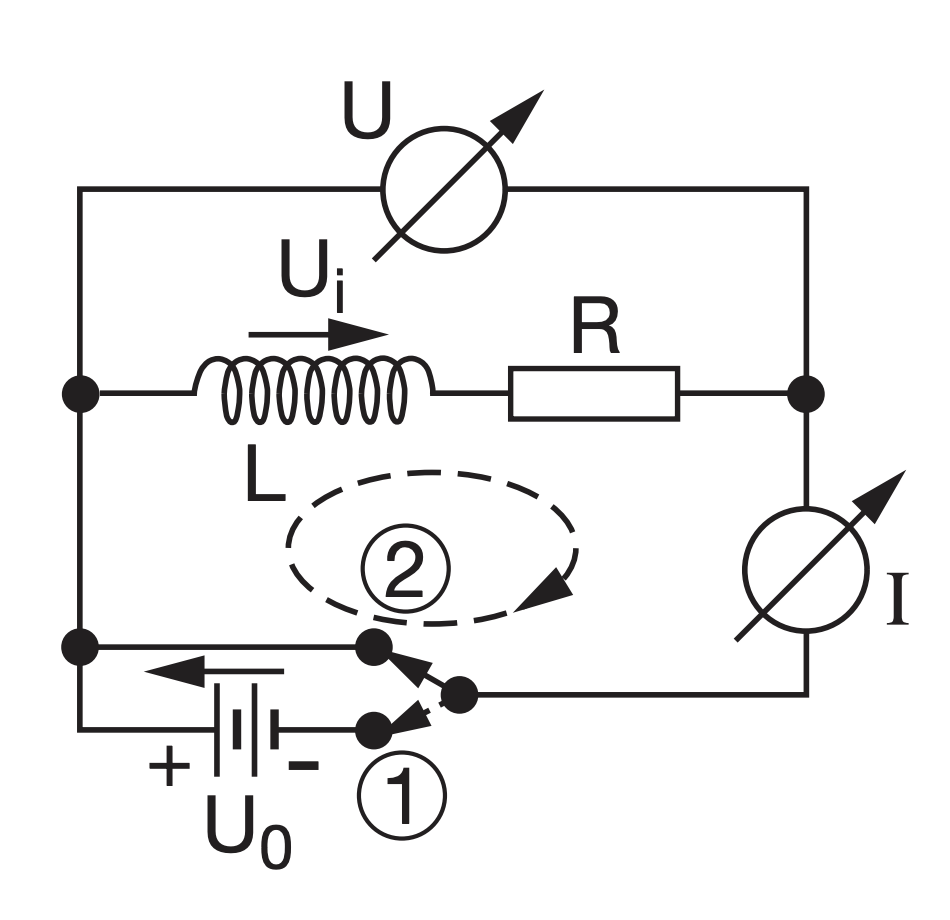
\includegraphics[scale=0.2]{Images/Schaltkreissmitspule.png}
    \end{center}
    Beim Einschalten der Batterie-Spannung $U_0$ ist die Induktionsspannung $U_i$ so gepolt, dass sie den Stromfluss zu behindern versucht (Lenz’sche Regel, Minuszeichen in der Gleichung). Beim Ausschalten versucht sie, die Abnahme des Stroms zu behindern.\\\\
    Einschalten:
    \[\quad I_0 = \frac{U_0}{R}\]
    \[U_0 - L\,\frac{dI}{dt} = I\,R\]
    \[I(t) = I_0\Bigl(1 - e^{-\frac{R}{L}(t - t_e)}\Bigr)\]\\
    
    Ausschalten:
    \[-L\,\frac{dI}{dt} = I\,R\]
    \[I(t) = I_0\,e^{-\frac{R}{L}(t - t_e)}\]
    \begin{center}
        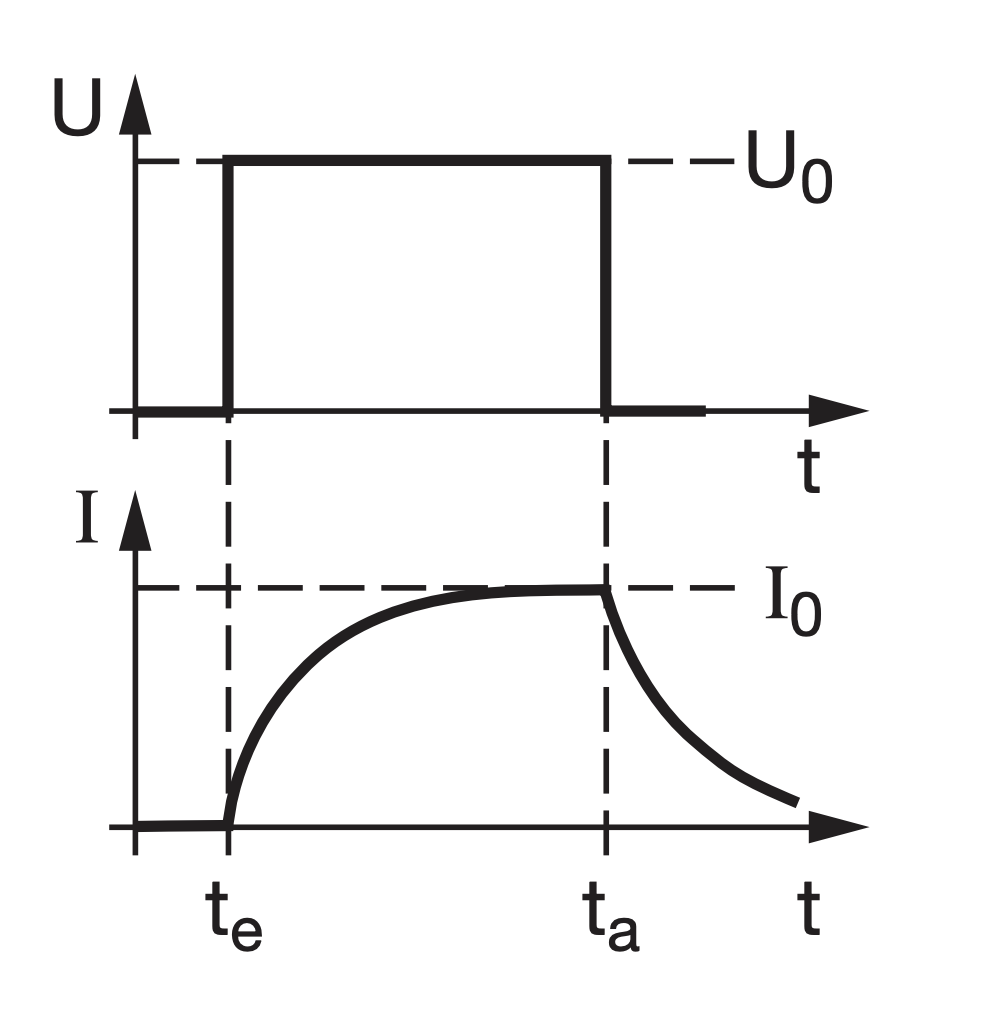
\includegraphics[scale=0.2]{Images/diagrammmitsspule.png}
    \end{center}
    Zeitliche Verzögerung wegen Selbstinduktion.
   




%=====================================================================================================================
\subsection{Materie im magnetischen Feld}
    Im Vakuum: $B_0 = \mu_0\,H_0$\\
    In Materie:
    \[B_m = \mu\,\mu_0\,H_0 = \mu\,\mu_0\,H_m\]
    \[\int U_{ind} dt |_m =  \mu \int U_{ind} dt |_o \]
    $\mu$ = Permeabilität des Materials.\\

    Suszeptibilität:\\
    $\chi_m = \mu - 1$ (Maß für Magnetisierung).\\\\
    Magnetisierung der Materie:
    \[\vec M = \chi_m\,\vec H\]
    
    \subsubsection{Diamagnetische Materialien}
        (Kämpft M-Feld)
        Im Inneren induziertes Feld ist dem äußeren Feld entgegengesetzt. $X < 0$, temperatur- und feldunabhängig. Beispiel: Supraleiter schwebt über Magnet.
        \begin{center}
            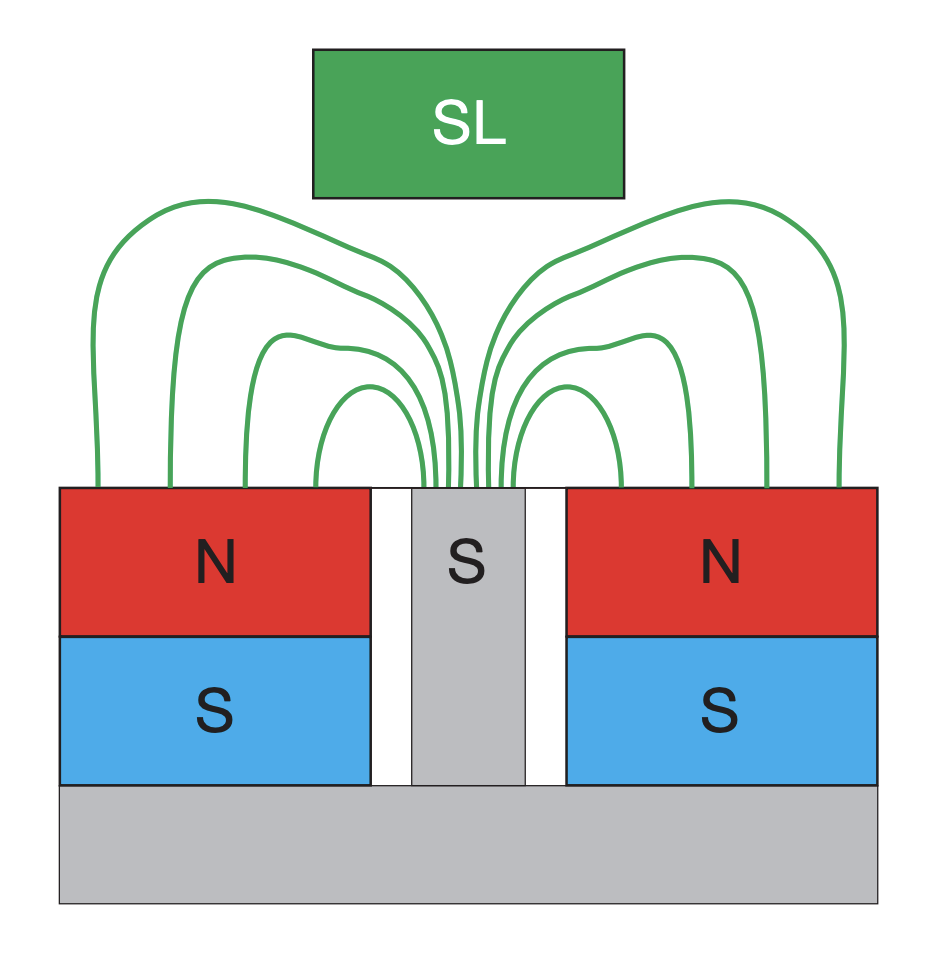
\includegraphics[scale=0.2]{Images/Suprameter.png}
        \end{center}
    \subsubsection{Paramagnetische Materialien}
        (Hilf M-Feld)
        $X > 0$
        Im Inneren induziertes Feld ist parallel zum äußeren Feld. Feldunabhängig und temperaturabhängig.
    \subsubsection{Ferromagnetische Materialien}
        Temperatur- und feldabhängig. Suszeptibilität: $\chi_m \approx \frac{1}{T - T_c}$, wobei $T_c$ = Curie-Temperatur.

\columnbreak
%%%%%%%%%%%%%%%%%%%%%%%%%%%%%%%%%%%%%%%%%%%%%%%%%%%%%%%%%%%%%%%%%%%%%%%%%%%%%%%%%%%%%%%%%%%%%%%%%%%%%%%%%%%%%%%%%%%%%%%%%%%%%%%%%%%%%%%%%%%%%%%%%%%%%%%%%%%%%%%%%%%%%%%%%%%%%%%%%%%%%%%%%%
\section{Wechselstrom}
\textit{(Hinweis: Es ist immer nur der Realteil physikalisch relevant, daher muss dies nicht extra angegeben werden.)}
%=====================================================================================================================
\subsection{Wechselstrom und Wechselspannung}
Strom:\\
\[
I(t) = \text{Re}(\tilde{I}(t)) = \text{Re}\left(I_0 (\cos(\omega t) + i \sin(\omega t))\right) = \text{Re}(I_0 e^{i\omega t})
\]\\

Die zugehörige Wechselspannung kann ebenso als komplexe Funktion dargestellt werden:
\[
U(t) = \omega B_0 A_0 \sin(\omega t) = U_0 \sin(\omega t)
\]
Dabei ist $\omega$ die Kreisfrequenz\\
$B_0$ das Magnetfeld\\
$A_0$ die Fläche einer Spule oder eines Systems.\\
Die Frequenz ist mit $\omega = 2\pi f$ gegeben, wobei $f$ die Frequenz in Hz ist.
%=====================================================================================================================
\subsection{Impedanz}

Die Impedanz $\tilde{Z}$ verallgemeinert den Widerstand im Wechselstromkreis:
\[
\tilde{Z} = R + iX = |\tilde{Z}| e^{i\varphi}
\]
mit
\[
|\tilde{Z}| = \sqrt{R^2 + X^2}, \quad \tan(\varphi) = \frac{X}{R}
\]
%=====================================================================================================================
\subsection{Phasenverschiebung zwischen $\tilde{U}$ und $\tilde{I}$}

\[
\tilde{U}(t) = \tilde{Z} \tilde{I}(t) = |\tilde{Z}| e^{i\varphi} \tilde{I}(t)
\]
Dies bedeutet, dass die Spannung um einen Winkel $\varphi$ gegenüber dem Strom verschoben ist.
%=====================================================================================================================
\subsection{Schaltungen}

Die Gesamtimpedanz hängt von der Schaltungsart ab:\\

\textbf{Reihenschaltung (Serie):}
\[
\tilde{Z}_{\text{tot}} = \sum_i \tilde{Z}_i
\]

\textbf{Parallelschaltung:}
\[
\frac{1}{\tilde{Z}_{\text{tot}}} = \sum_i \frac{1}{\tilde{Z}_i}
\]
\textbf{Knotenregel:} 
\[
\sum_k \tilde{I}_k(t) = 0
\]

\textbf{Maschenregel:} 
\[
\underbrace{\sum_i \tilde{U}_i(t)}_{\text{batt}} 
\quad - \quad 
\underbrace{\sum_k \tilde{Z}_k \tilde{I}_k(t)}_{\text{abfalle eine Masche}} 
= 0
\]
%=====================================================================================================================
\subsection{Leistung im Wechselstromkreis}

Die komplexe Leistung ergibt sich aus:
\[
\tilde{P} = \tilde{I} \tilde{U}
\]

Für die mittlere (effektive) Leistung gilt:
\[
\bar{P} = \frac{1}{2} \text{Re}(\tilde{I} \bar{\tilde{U}}) = \frac{1}{2} I_0 U_0 \cos(\varphi)
\]
%=====================================================================================================================
\subsection{ Widerstand ($R$)}

\textbf{Spannung:}
\[
\tilde{U}(t) = R \tilde{I}(t) = R I_0 e^{i\omega t}
\]

\[
\tilde{Z}_R = R  \quad (\varphi = 0)
\]

\textbf{Leistung:}
\[
P(t) = R [\tilde{I}(t)]^2 = \frac{1}{2} R I_0^2 (1 - \cos^2 \omega t)
\]
\[
\bar{P} = \frac{1}{2} R I_0^2
\]
%=====================================================================================================================
\subsection{ Spule ($L$)}

\textbf{Spannung:}
\[
\tilde{U}(t) = L \frac{d\tilde{I}}{dt} = i \omega L I_0 e^{i\omega t}
\]
\[
\tilde{Z}_L = i\omega L \ (\varphi = \frac{\pi}{2})
\]

\textbf{Leistung:}
\[
P(t) = \frac{1}{2} \omega L I_0^2 \sin(2\omega t)
\]
\[
\bar{P} = 0
\]
%=====================================================================================================================
\subsection{Kondensator ($C$)}

\textbf{Spannung:}
\[
\tilde{U}(t) = \frac{Q}{C} = \frac{1}{C} \int \tilde{I}(t) \, dt = \frac{1}{i\omega C} I_0 e^{i\omega t}
\]
\[
\tilde{Z}_C = \frac{1}{i\omega C} = \frac{-i}{\omega C} \ (\varphi = -\frac{\pi}{2})
\]

\textbf{Leistung:}
\[
P(t) = -\frac{1}{2} \frac{I_0^2}{\omega C} \sin(2\omega t)
\]
\[
\bar{P} = 0
\]

%=====================================================================================================================
\subsection{Trasformator}
\begin{center}
    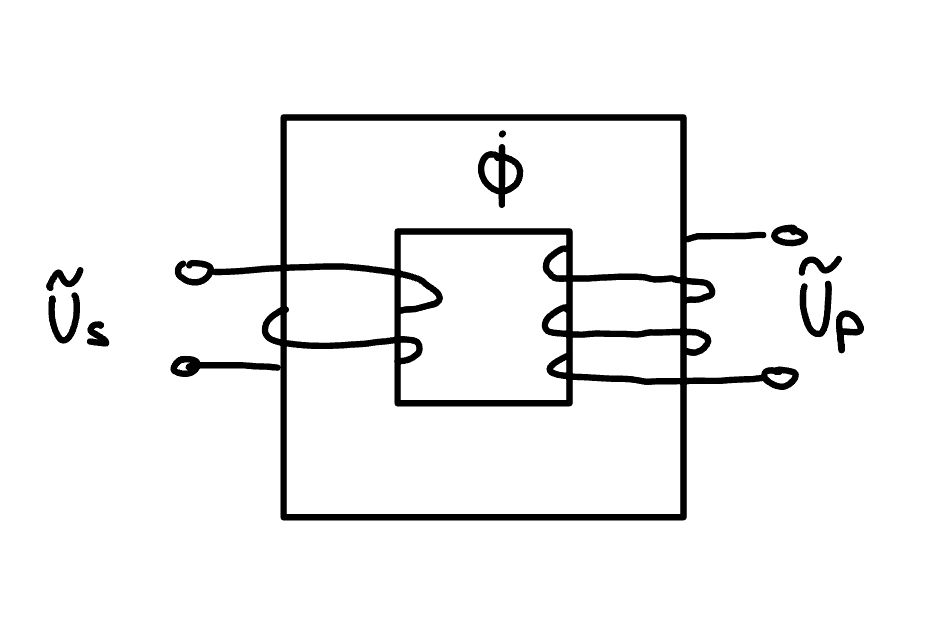
\includegraphics[scale=0.1]{Images/transformator.jpg}
\end{center}
\[
|\frac{\tilde{U}_p}{\tilde{U}_s}| = \frac{N_s}{N_p}
\]

\begin{itemize}
    \item \( U_p \): Primärspannung\\
    \item \( U_s \): Sekundärspannung\\
    \item \( N_p \): Anzahl der Windungen der Primärspule\\
    \item \( N_s \): Anzahl der Windungen der Sekundärspule
\end{itemize}







\columnbreak
%%%%%%%%%%%%%%%%%%%%%%%%%%%%%%%%%%%%%%%%%%%%%%%%%%%%%%%%%%%%%%%%%%%%%%%%%%%%%%%%%%%%%%%%%%%%%%%%%%%%%%%%%%%%%%%%%%%%%%
\section{Wellen}

%=====================================================================================================================
%=====================================================================================================================
\subsection{Wellenfunktion und Wellengleichung}
Ebene Welle der Form:
\[
\Psi(r,t) = A \cos(\omega t - k r)
\]
mit \(r \in \{x,y,z\}\).\\

\textbf{Wellenparameter:}
\[
T = \frac{2\pi}{\omega}, \quad
k = \frac{2\pi}{\lambda}, \quad
\omega = 2\pi f = \frac{2\pi}{T}
\]

Amplitude: \(A\)\\
Knotenabstand: \(d = \frac{\lambda}{2}\)\\
Seillänge: \(l = n \cdot \frac{\lambda_n}{2}\)\\
Grundschwingung: \\

\textbf{Ausbreitungsgeschwindigkeit (harmonische Welle):}
\[
v_{\text{ph}} = \frac{\omega}{k} = \lambda f = \sqrt{\frac{\sigma}{\rho}}
\]\\
\(\rho\): Massendichte [kg/m\(^3\)]\\
\(\sigma\): Seilspannung [N/m\(^2\)], wobei \(F = \sigma \cdot A_{\text{Querschnitt}}\)\\

\textbf{Gruppengeschwindigkeit:}
\[
v_{\text{gr}} = \frac{d\omega}{dk} \neq v_{\text{ph}}
\]

\textbf{Maximale Geschwindigkeit eines Teilchens:}
\[
v_{\text{max}} = A \omega
\]

\textbf{Wellengleichung:}
\[
\frac{\partial^2 \Psi(r,t)}{\partial t^2} = v_{\text{ph}}^2 \cdot \frac{\partial^2 \Psi(r,t)}{\partial r^2}
\]\\

\textbf{Intensität (Energiestromdichte):}
\[
I = |\vec{j}_E| = |\rho_E \cdot \vec{v}_{\text{ph}}|
\]
\(\vec{j}_E\): vektorielle Energiestromdichte\\
\(\rho_E\): Energiedichte\\
\[
I \sim A^2
\]

\subsection{Wellenfunktion und Wellengleichung}
    Ebene Welle der Form:
    \[\Psi(r,t) = A \cos(\omega t - k r)\]
    mit \(r \in \{x,y,z\}\).\\
    
    Periodendauer \(T = \frac{2\pi}{\omega}\).\\
    Wellenzahl \(k = \frac{2\pi}{\lambda}\).\\
    Winkelgeschwindigkeit \(\omega = 2\pi f = \frac{2\pi}{T}\).\\
    Amplitude \(A\).\\
    Knotenabstand \(d = \frac{\lambda}{2}\).\\
    Seillänge \(l = n\,\frac{\lambda_n}{2}\).\\
    Grundschwingung: \(\lambda = 2\,l\).\\



    Ausbreitungsgeschwindigkeit (Harmonische Wellen):
    \[v_{ph} =  \frac{\omega}{k} = \frac{2\pi f}{k} = \lambda\,f = \sqrt{\frac{\sigma}{\rho}}\]\\
    \(\rho\) = Massendichte [kg/m\(^3\)]\\
    \(\sigma\) = Seilspannung [N/m\(^2\)].\\
    ($F = \sigma \cdot A_{\text{Querschnitt}}$)\\
    Gruppengeschwindigkeit:
    \[V_{gr} = \frac{dw}{dk}\]
    Maximale Geschwindigkeit eines Teilchens auf dem Medium:
    \[v_{\text{max}} = A\,\omega\]


    Wellengleichung:
    \[\frac{\partial^2 \Psi(r,t)}{\partial t^2} = v_{ph}^2 \,\frac{\partial^2 \Psi(r,t)}{\partial r^2}.\]
    \\
    Intensität (Energiestromdichte):
    \[I = |\vec j_E| = |\rho_E\,\vec v_{ph}|\]\\
    \(\vec j_E\) die vektorielle Energiestromdichte\\
    \(\rho_E\) die Energiedichte\\
    \(I \sim A^2\).\\



%=====================================================================================================================
\subsection{Superposition Wellen}
    Ebene Wellen der Form:\\
    in positive Richtung:
    \[\Psi_{\rightarrow}(r,t) = A \cos(\omega t - k r)\] 
    in negative Richtung:
    \[\Psi_{\leftarrow}(r,t) = A \cos(\omega t + k r)\] 
    mit \(r \in \{x,y,z\}\).\\

    Superposition:
    \[\Psi = \Psi_{\rightarrow} + \Psi_{\leftarrow}\]

    \[\Psi = 2A \sin(k r) \cos(\omega t).\]

    Superposition von zwei Wellen mit verschiedenen Frequenzen und Wellenzahlen:
    \[\Psi = 2A \cos\Bigl(\tfrac{\Delta \omega}{2}t - \tfrac{\Delta k}{2} r\Bigr) \cos\bigl(\overline{\omega}t - \overline{k} r\bigr).\]


%=====================================================================================================================
\subsection{Dopplereffekt}
\subsubsection{Beobachter bewegt, Quelle ruhend}
\paragraph{Beobachter bewegt sich auf die Quelle zu}
\[\boxed{f_B =f_Q \Bigl(1 + \tfrac{v_B}{c}\Bigr)}\]
wobei \(f_B > f_Q\).\\

\paragraph{Beobachter entfernt sich von der Quelle}
\[\boxed{f_B = f_Q \Bigl(1 - \tfrac{v_B}{c}\Bigr)}\]
wobei \(f_B < f_Q\).\\

\subsubsection{Beobachter ruht, Quelle bewegt}
\paragraph{Quelle bewegt sich auf den Beobachter zu}
\[\boxed{f_B = f_Q \,\frac{1}{1 - \tfrac{v_Q}{c}} = f_0 \sum_{k=0}^{\infty} \Bigl(\tfrac{v_Q}{c}\Bigr)^k}\]
wobei \(f_B > f_Q\).\\

\paragraph{Quelle entfernt sich}
\[\boxed{f_B = f_Q \,\frac{1}{1 + \tfrac{v_Q}{c}} = f_0 \sum_{k=0}^{\infty} \bigl(-\tfrac{v_Q}{c}\bigr)^k}\]

\subsubsection{Beobachter bewegt, Quelle bewegt}
\paragraph{Bewegen sich aufeinander zu}
\[\boxed{f_B = f_Q \,\frac{c + v_B}{c - v_Q}}\]
wobei \(f_B > f_Q\).\\

\paragraph{Bewegen sich voneinander weg}
\[\boxed{f_B = f_Q \,\frac{c - v_B}{c + v_Q}}\]
wobei \(f_B < f_Q\). \\


%=====================================================================================================================
\subsection{Dopplereffekt des Lichtes im Vakuum}
\subsubsection{Bewegen sich aufeinander zu}
\[\boxed{f_B = f_Q \,\sqrt{\frac{1 + \beta}{1 - \beta}}}\]
wobei \(f_B > f_Q\).\\

\subsubsection{Bewegen sich voneinander weg}
\[\boxed{f_B = f_Q \,\sqrt{\frac{1 - \beta}{1 + \beta}}}\]
wobei \(f_B < f_Q\). \\
mit \(\beta = \frac{v}{c}\)

\columnbreak
%%%%%%%%%%%%%%%%%%%%%%%%%%%%%%%%%%%%%%%%%%%%%%%%%%%%%%%%%%%%%%%%%%%%%%%%%%%%%%%%%%%%%%%%%%%%%%%%%%%%%%%%%%%%%%%%%%%%%%
\section{Elektromagnetische Wellen}
\begin{center}
    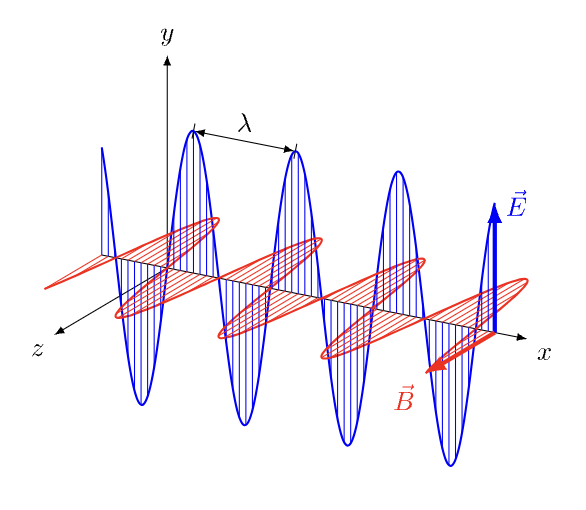
\includegraphics[scale=0.38]{Images/elektrowellen.png}
\end{center}

    Im Vakuum mit Lichtgeschwindigkeit:
    \[c = \frac{1}{\sqrt{\varepsilon_0 \,\mu_0}} = \lambda\,f = 3 \times 10^8 \,\frac{\text{m}}{\text{s}}\]

%=====================================================================================================================
\subsection{Abstrahlung von Hertzschen Dipols}
    Elektromagnetische Wellen entstehen durch bewegte elektrische Ladung.\\
    a) Die von einem Dipol (Hertz’scher Dipol) ausgehende Strahlung ist linear polarisiert.\\
    b) In Richtung der Antennenachse (x) wird keine Energie abgestrahlt.\\

    Ein Hertz’scher Dipol basiert auf dem Prinzip eines schwingenden LC-Kreises: Ladungen schwingen zwischen Kondensator und Spule → schwingender Dipol.
    \[\vec p  = q \vec l = \vec p_0 \cos(\omega t) \]
%=====================================================================================================================
\subsection{Wellengleichung}
    Ebene EM-Wellen:
    \[\vec E = \vec E_0 \cos(\omega t - k r)\]
    \[\vec H = \vec H_0 \cos(\omega t - k r)\]\\

    Die Welle breitet sich in $r$-Richtung aus.\\
    Ausbreitungsgeschwindigkeit:
    \[v_{ph} = \frac{\omega}{k} = \lambda\,f = c.\]
    \[\frac{\partial^2 \Psi(t,r)}{\partial t^2} = \frac{1}{\varepsilon_0 \,\mu_0} \,\frac{\partial^2 \Psi(t,r)}{\partial r^2}\]\\
    \[\frac{1}{\varepsilon_0 \,\mu_0} = c^2\]\\
    \[B_0 = \frac{E_0}{c}\]

%=====================================================================================================================
\subsection{Poynting-Vektor}
Beschreibt Richtung und Dichte des Energietransportes (Energieflussdichte) der elektromagnetischen Welle:
\[
\vec{S} = \vec{E} \times \vec{H} = \vec{J}_E
\]
$S = [\frac{W}{m^2}]$\\
\(\vec{S}\) ist senkrecht zu \(\vec{E}\) und \(\vec{H}\).\\

\textbf{Energiedichte:}
\[
\rho_E = \frac{1}{2} \varepsilon_0 E^2 + \frac{1}{2} \frac{B^2}{\mu_0}
\]

Für ebene Wellen im Vakuum gilt:
\[
|\vec{S}| = \rho_E \cdot c
\]

\textbf{Intensität (gemittelt über Zeit):}
\[
I = \langle |\vec{S}| \rangle = \frac{1}{2}\,\varepsilon_0\,E_0^2\,c
\]

\textbf{Energiefluss:}
\[
\bar{j}_E = \frac{1}{A} \cdot \frac{\Delta E_{\text{em}}}{\Delta t} = \rho_E \cdot \vec{v}_{\text{ph}}
\]

\textbf{Intuitive Abhängigkeit:}
\[
I \sim |\vec{j}_E| \sim S_0^2
\]

\textbf{Mechanische Analogie (harmonische Welle):}
\[
\Delta E_{\text{kin}} = \frac{1}{2} \Delta m \omega^2 s_0^2
\]

%=====================================================================================================================
\subsection{Poynting-Vektor}
Beschreibt Richtung und Dichte des Energietransportes (Energieflussdichte) der elektromagnetischen Welle:
\[
\vec{S} = \vec{E} \times \vec{H} = \vec{j}_E
\]
\[
[\vec{S}] = \left[\frac{W}{m^2}\right]
\]
\(\vec{S}\) ist senkrecht zu \(\vec{E}\) und \(\vec{H}\).\\

\textbf{Energiedichte:}
\[
\rho_E = \frac{1}{2} \varepsilon_0 E^2 + \frac{1}{2} \frac{B^2}{\mu_0}
\]

Für ebene Wellen im Vakuum gilt:
\[
|\vec{S}| = \rho_E \cdot c
\]
%%%%%%%%%%%%%%%%%%%%%%%%%%%%%%%%%%%%%%%%%%%%%%%%%%%%%%%%%%%%%%%%%%%%%%%%%%%%%%%%%%%%%%%%%%%%%%%%%%%%%%%%%%%%%%%%%%%%%%%%%%%%

\section*{Appendix}
\[\int \frac{1}{a x + b}\,dx = \frac{1}{a} \ln\bigl|a x + b\bigr| + C.\]

\[\nabla \times \vec E = 
\begin{pmatrix}
\partial_y E_z - \partial_z E_y \\
\partial_z E_x - \partial_x E_z \\
\partial_x E_y - \partial_y E_x
\end{pmatrix},
\quad
\Delta = \frac{\partial^2}{\partial x^2} + \frac{\partial^2}{\partial y^2} + \frac{\partial^2}{\partial z^2}.\]
Fläche Kugel:
\[A = 4\pi r^2,\quad V = \frac{4}{3}\pi r^3.\]
Fläche Zylinder:
\[A = 2\pi r h,\quad V = \pi r^2 h.\]
Kreissektor:
\[A = \frac{1}{2}r^2 \varphi,\quad \varphi = \omega t.\]

Steigung = \(\tan(\alpha)\).\\

Impuls: 
\[p = m\cdot v,\quad [p] = \frac{\text{kg}\,\text{m}}{\text{s}}.\]
\[p_{\text{max}} = m \cdot v_{\text{max}},\quad v_{\text{max}} = A \cdot \omega.\]
Keine Gegeninduktion, falls der Fluss konstant ist.\\

Transformator: Überträgt Leistung.\\

Jacobi-Matrix nicht vergessen!!!

\[
(\vec{a} \times \vec{b}) \cdot \vec{c}
= - (\vec{a} \times \vec{c}) \cdot \vec{b}
= - (\vec{b} \times \vec{a}) \cdot \vec{c}
= - (\vec{c} \times \vec{b}) \cdot \vec{a}
\]
\columnbreak
\subsection*{Einheiten}
\begin{empheq}{align*} % Dipolmoment???
        \vec{B}                              &\quad \text{Magnetische Induktion}             & \scriptstyle T = \frac{W b}{m^2} = \frac{V \cdot s}{m^2} = \frac{kg}{A \cdot s^2} \\
        C                                               &\quad \text{Kapazität}                         & \scriptstyle F = \frac{C}{V} = \frac{A \cdot s}{V} = \frac{A^2 \cdot s^4}{kg \cdot m^2} \\
        D                                               &\quad \text{elek. Flussdichte /}               & \scriptstyle \frac{A \cdot s}{m^2}\\
                                                        &\quad \text{Verschiebungsdichte}               & \\
        \vec{E}                              &\quad \text{e. Feld}                           & \scriptstyle \frac{N}{C} = \frac{V}{m} = \frac{kg \cdot m}{s^3 \cdot A} \\
        E                                               &\quad \text{Energie} \quad 1eV \cdot e = 1J    & \scriptstyle J = Nm = CV = Ws \frac{kg \cdot m^2}{s^2} \\
        \scriptstyle f = \nu = \frac{1}{T}              &\quad \text{Frequenz}                          & \scriptstyle \frac{1}{s} = Hz \\
        \vec{F}                              &\quad \text{Kraft}                             & \scriptstyle N = \frac{V \cdot C}{m} = \frac{kg \cdot m}{s^2} \\
        \vec{H}                              &\quad \text{magn. Feldstärke}                  & \scriptstyle \frac{A}{m} \\
        \vec{I}                              &\quad \text{el. Strom}                         & \scriptstyle A = \frac{C}{s} \\
        \scriptstyle \vec{j} = \frac{I}{A}   &\quad \text{Stromdichte}                       & \scriptstyle \frac{C}{s \cdot m^2} \\
        k                                               &\quad \text{Federkonstante}                    & \scriptstyle \frac{N}{m} \\
        L                                               &\quad \text{Induktivität}                      & \scriptstyle H = \frac{T \cdot m^2}{A} = \frac{V \cdot s}{A} \\
                                                        &                                               & \scriptstyle = \frac{kg \cdot m^2}{A^2 \cdot s^2} \\
        P                                               &\quad \text{Leistung}                          & \scriptstyle W = V \cdot A = \frac{J}{s} \\
        Q                                               &\quad \text{Ladung}                            & \scriptstyle C = A \cdot s \\
        R                                               &\quad \text{el. Widerstand}                    & \scriptstyle \Omega = \frac{V}{A} \\
        S                                               &\quad \text{Siemens}                           & \scriptstyle S = \frac{1}{\Omega} = \frac{A}{V} \\
        T                                               &\quad \text{Periodendauer /}                   & \scriptstyle s \\
                                                        &\quad \text{Schwingungsdauer}                  & \\
        U                                               &\quad \text{Potentialdiff. / Spannung}         & \scriptstyle V = \frac{W}{A} = \frac{J}{C} \\
                                                        &                                               & \scriptstyle = \frac{Nm}{As} = \frac{kg \cdot m^2}{A \cdot s^3} \\
        \vec{v}                              &\quad \text{Geschwindigkeit}                   & \scriptstyle \frac{m}{s} \\
        W                                               &\quad \text{Arbeit}                            & \scriptstyle J = N \cdot m \\
                                                        &                                               & \scriptstyle = \frac{kg \cdot m^2}{s^2} = C \cdot V \\
        Z                                               &\quad \text{Impedanz}                          & \scriptstyle \Omega = \frac{V}{A} = \frac{kg \cdot m^2}{A^2 \cdot s^3} \\
        \varepsilon                                     &\quad \text{Dielektrizitätskonst. Mat.}        & \scriptstyle \frac{C}{V \cdot m} = \frac{A \cdot s}{V \cdot m} \\
        \Psi_E                                          &\quad \text{elek. Fluss}                       & \scriptstyle V \cdot m = \frac{N \cdot m^2}{C} \\
        \Phi_M                                          &\quad \text{magn. Fluss}                       & \scriptstyle Wb = T \cdot m^2 \\
        \Phi                                            &\quad \text{elek. Potential}                   & \scriptstyle [-] \\
        \lambda = \frac{c}{f}                           &\quad \text{Wellenlänge}                       & \scriptstyle m \\
        \mu                                             &\quad \text{magn. Feldk. /}                    & \scriptstyle \frac{V \cdot s}{A \cdot m} \\
                                                        &\quad \text{Permeabilität}                     & \\
        \rho                                            &\quad \text{spez. Widerstand}                  & \scriptstyle \Omega \cdot m \\
        \omega = 2 \pi f                                &\quad \text{Kreisfrequenz}                     & \scriptstyle s^{-1} = Hz \\
        %&\quad \text{} & \scriptstyle  \\
        \end{empheq}

        \begin{empheq}{align*}
        &\textbf{Kräfte}\\
        F                           &\quad \text{Kraft Allgemein}           & \scriptstyle = m \cdot a\\
        F_g                         &\quad \text{Gewichtskraft}             & \scriptstyle = m \cdot g\\
        F_\text{Fed}                &\quad \text{Federkraft}                & \scriptstyle = R \cdot s\\
        F_Z                         &\quad \text{Zentripetalkraft}          & \scriptstyle = m \frac{v^2}{r} = m \omega^2 r \\
        &\textbf{Energie}\\
        E                           &\quad \text{Energie Allgemein}         & \scriptstyle = \vec{F} \cdot \vec{s}\\
        E_\text{pot}                &\quad \text{Potentielle Energie}       & \scriptstyle = m \cdot g \cdot h\\
        E_\text{kin}                &\quad \text{Kinetische Energie}        & \scriptstyle = \frac{1}{2} m \cdot v^2\\
        W = \Delta E                &\quad \text{Zusammenhang Arbeit Energie}\\

        \end{empheq}




\end{multicols*}
\end{document}
